\begin{refsection}
\chapter{Theory and Background}
\label{ch:theory_and_background}
In this chapter, the necessary methodologies and theoretical footing necessary for later chapters is established. Additionally, background into the application of diamond within the context of power electronics engineering is given to assist in the progression from electronics to diamond electronics.
\section{Electronics Background}
\subsection{Introduction}
Electronic devices based on semiconductors are the backbone of modern technology, long since replacing vacuum-tube based devices in power electronics and consumer electronic applications. As implied by the name, power electronic devices in particular deal with applications where the conversion and control of electrical power is concerned. Over the past half a century, the global electrical consumption has slowly, and continuously grown. Between 1980 and 2022, electrical consumption rose from 7300 to 25,000 terawatt-hours \cite{enerdata2023net}. This is likely to increase ever further, with the electricity consumption due to data centres, artificial intelligence (AI) and cryptocurrency sectors predicted to double by 2026 \cite{IEA2024}. This is supported in large by the significant growth in renewable energy sources, which are set to provide more than a third of total electricity generation globally by early 2025, overtaking the market share of coal.

When it comes to the power electronics themselves, a mix of silicon-based devices with more recent wide bandgap substrates such as GaN and SiC are the most advanced solutions for power applications that range from high voltage direct current (HVDC) converter stations to flexible ac transmission system (FACTS) devices. These devices are used for variable-speed drivers in motors, the regulation of ac power grids and more recently throughout the electric vehicle (EV) market in the form of EV battery chargers in particular \cite{Tolbert2005, Afonso2020}. Depending on the application, various blocking voltages and maximum operating frequencies can be readily acquired.

\begin{table}[H]
\centering
\begin{tabular}{|c|c|c|c|c|c|c|c|}
\hline
ID          & Type & x (\si{\milli\metre}) & $V_{B}$ (\si{\kilo\volt}) & F (\si{\kilo\hertz}) & I (\si{\kilo\ampere}) & $R_{t}$ (\si{\kelvin\per\kilo\watt}) & $T_{max}$ (°C)  \\ \hline

T1503             & Thyristor & 150 & 8   & 0.06  & 55  & 6.3  & 120   \\ \hline
DZ950                & Diode     & 70  & 4.4   & 0.06  & 29  & 42   & 150   \\ \hline
TT240               & Thyristor & 60  & 3.8 & 0.05   & 6.1  & 39  & 125    \\ \hline
D2601               & Diode    & 121  & 9   & 0.06  & 52   & 8.9    & 160    \\ \hline
AIKQ120        & IGBT     & 16   & 750    & 4.1  & 0.36    & 170   & 175    \\ \hline
\end{tabular}
\caption{A sample of readily available current power electronic devices, as sourced from Infineon Technologies AG \cite{infineon:T1503N, infineon:DZ950N, infineon:TT240N, infineon:D2601N, infineon:AIKQ120N75CP2}.}
\label{tab:components}
\end{table}

Table \ref{tab:components} summarises a small sample of current power electronic devices. In this table, x is is the approximate diameter (thyristors are in a circular package, diodes and IGBT's are in a rectangular package), $V_{B}$ is the maximum reverse bias or blocking voltage, F is the estimated maximum operating frequency, I is the maximum forward surge current, $R_{t}$ is the maximum thermal resistance from junction to case and $T_{max}$ is the maximum operating junction temperature. The exact type of device used will always be a trade-off, while thyristors of up to 10~\si{\kilo\volt} are available, these devices inevitably require a significantly larger junction size, which increases the challenge of thermal management solutions, the cost of such devices overall, and also raises the complexity of such devices. While variations of thyristors such as the integrated gate-commutated thyristor (IGCT) or gate turn off (GTO) thyristors both allow for higher operating frequencies of between 0.1--1~\si{\kilo\hertz}, this comes at the expense of a lower blocking voltage and peak surge current rating. IGCT or GTOs are widely used within motor control, renewable energy management and anywhere with large power draws like in rail travel \cite{Tolbert2005}. In the case of power inverters, where fast switching frequency is necessary, insulated gate bipolar transistors (IGBT) due to the ideal balance between breakdown voltage and operating frequency offered. For smaller systems such as conventional power supplies, amplifiers and consumer electronics in general, less specific transistors such as metal oxide semiconductor field effect transistors (MOSFETs), junction field effect transistors (JFETs) and bipolar junction transistors (BJTs) are in wide usage.

Silicon based devices are limited by a few key factors. First, the low thermal conductivity of silicon and narrow bandgap limit operating temperatures to around 150\si{\degreeCelsius}. Second is the critical electric field of silicon, which is around 0.3~\si{\mega\volt\per\centi\metre} \cite{McCluskey1996-rz}. Due to the low critical electric field of silicon, there is a need for series stacking of silicon based devices with complex triggering systems to ensure that the potential bias across any single junction does not exceed the critical electric field \cite{ZhiweiLiu2010, Tolbert2005}. Finally, as a result of both the requirement for stacked silicon devices and also advanced thermal management solutions, the electrical power losses can rise significantly.

\subsection{Wide Bandgap Semiconductors}
A key solution to the issues faced by silicon power electronics is to utilise a wide-bandgap semiconductor. In particular, Si can be compared to silicon carbide (SiC), gallium nitride (GaN), gallium oxide (\ce{Ga2O3}) and diamond. All of these materials have larger critical electric fields and higher thermal conductivities, significantly improving the viability of devices based on single structures in contrast to the series stacking of Si. Diamond stands apart from these comparators, with a critical field 30 times higher than Si and 3 times higher than SiC \cite{Zaitsev2010-vd}. The maximum carrier mobility of diamond is another best in class comparison, with intrinsic carrier mobilities of 4500 and 3800 ~\si{\centi\metre\squared\per\volt\per\second} for electrons and holes respectively \cite{Isberg2002}. Diamond's thermal conductivity is similarly high, at 2200~\si{\watt\per\metre\kelvin}, and also has a relative dielectric constant of 5.7 \cite{Zaitsev2010-vd}. To compare differing materials figures of merit (FOM) are typically used. In the case of diamond, two important FOMs were introduced by Baliga \cite{Baliga1989}. First is the Baliga FOM (BFOM), given by:
\begin{equation}
    BFOM = \epsilon_{r}\mu E_{max}^{3}
\end{equation}
where $\epsilon_{r}$ is the relative dielectric constant, $\mu$ is the carrier mobility and $E_{max}^{3}$ is the breakdown field, typically given in units of \si{\mega\volt\per\centi\metre}. The second is Baliga's high-frequency FOM (BHFOM), using the same notation:
\begin{equation}
    BHFOM = \mu E_{max}^{2}
\end{equation}
\noindent While the BFOM is used to estimate the trade off between conductive losses and breakdown voltage for a unipolar device, the BHFOM is used to include switching losses associated with a gate capacitance, as in FET's. There are further FOM's, but for the comparison of materials presented here, the BFOM and BHFOM are used.

\begin{table}[htbp]
\centering
\caption{Material properties and figures of merit (FOM) for various semiconductors \cite{Saslow1966, Yu2010, sze2006, Schroder2006-sx}.}
\label{tab:material_properties}
\begin{tabular}{@{}|c|c|c|c|c|c|c|@{}}
\hline
& & \textbf{Si} & \textbf{4H-SiC} & \textbf{GaN} & \textbf{\ce{Ga2O3}} & \textbf{Diamond} \\ 
\hline
$E_{g}$ (\si{\electronvolt}) & &1.12&3.20&3.45 &4.9 &5.47 \\
$v_{s}$ ($10^{7}$~\si{\centi\metre\squared\per\volt\per\second}) & e- & 1.1& 1.9 & 2.5& 2& 2.5, 1.9 \cite{Pomorski2007, Pomorski2008}\\
& h+& 0.8& 1.2& - & - & 1.0, 1.4 \cite{Pomorski2007}\\
$\mu$ (\si{\centi\metre\squared\per\volt\per\second})& e-& 1500 & 1000& 1500& 300& 4500 \cite{Isberg2002}\\
& h+& 450& 120& 200& -& 3800\cite{Isberg2002}\\
$E_{max}$ (\si{\mega\volt\per\centi\metre})& & 0.3& 2.8& 5& 8& 10--22\cite{Volpe2010}\\
$\epsilon_{r}$& & 11.9& 9.66& 8.9& 9.93& 5.7 \cite{Zaitsev2010-vd}\\
$\gamma$ (\si{\watt\per\metre\per\kelvin})& &150 &490 &130 &23 &2200 \cite{Zaitsev2010-vd}\\
BFOM& & 1.0& 440& 2950& 3516& 3380--473078\\
BHFOM& & 1.0& 58& 237& 158& 1486--12510\\
\hline
\end{tabular}
\end{table}

Table \ref{tab:material_properties} provides the relevant material properties and the two FOM's for all materials. In this table, $\gamma$ is used to represent the thermal conductivity, and the second column is used to denote electrons (e-) or holes (h+) for the material properties that require this distinction, namely the saturation drift velocity $v_{s}$ and carrier mobility $\mu$. As the electrical properties of diamond are quite dependent upon the crystal structure, with defect centres strongly impacting the carrier mobility due to the rise in coulombic scattering events, it is typical go give a range of FOMs for diamond, which helps to represent the range of crystal dependent properties. At the low end, highly defective, disordered diamond with low carrier velocities and critical electric fields is considered. While at the high end, electronic grade diamond with less than 5 parts per billion nitrogen defect centres and highly oriented single crystal growth is used to represent the peak upper limit. These properties are also orientation specific \cite{Milln2012}, due in part to differing rates of compensation within doped diamond films \cite{pinault2021, stenger2021}, so care must be taken in the selection of crystal substrate if a high FOM is required.

\subsection{Characterisation Techniques}
In the following sections, an overview of the general principles behind characterisation techniques used throughout the experimental work in this thesis are given.

\subsubsection{TLM}
\label{subsubsection:ltlm_explained}

The Transmission Line Method (TLM) is widely used for evaluating the contact resistivity between metal and semiconductor regions, especially when the semiconductor region is isolated from the substrate by a junction. This technique, however, faces challenges when the junction isolation is leaky, potentially resulting in incorrect parameter extraction due to parasitic leakage currents.

\paragraph{Basic Assumptions and Limitations}
TLM assumes a uniform sheet resistance, an isotropic interface between conducting regions and current flow restriction to the channel of interest.

These assumptions may not hold in certain cases, such as in GaN/AlGaN two-dimensional electron gas systems where the sheet resistance under the contact area varies, leading to discrepancies in applying standard TLM equations for contact resistivity determination \cite{Bystrova2017}.

\paragraph{Assumptions}
The core assumption in TLM is that the metal’s resistivity in the contact is negligible compared to the contact resistivity, thus simplifying the resistance of a single contact to primarily \(R_{c}\). Under this assumption, total resistance can be expressed and analysed by constructing test structures of varying lengths and measuring the resultant resistance. By plotting these resistances against the length and extrapolating to zero length, the intercept gives twice the contact resistance, and the slope provides the sheet resistance of the semiconductor.

\paragraph{Contact Resistivity and Current Crowding}
Specific contact resistivity (\(\rho_{c}\)) is defined as \(\rho_{c} = A \cdot R_{c}\), where \(A\) is the contact area. It is critical to differentiate between physical and effective contact areas due to the non-uniformity of current flow, a phenomenon known as current crowding. Current crowding, particularly pronounced near the edges of the contact, leads to a variation in the effective current distribution.

\paragraph{LTLM Theory}
\begin{equation}
    R_{T}=2R_{m}+2R_{c}+R_{semi}
\end{equation}
The core derivation of linear TLM theory derives from the observation that total resistance $R_{T}$ is made up of two contact resistances $R_{c}$, two resistances due to wires in the circuits/probes $R_{m}$, and one resistance of the semiconductor in question $R_{semi}$. By measuring the total resistance across differing channel lengths, with known areas of metal contacts to the semiconductor, it is possible to derive the following \cite{Schroder2006-sx}:

\begin{equation}
    R_{T} = \frac{R_{sh}}{W}d+2R_{c}
\end{equation}
where $R_{sh} = \frac{R_{semi}W}{d}$ is the sheet resistance, $W$ is the width of the contacts and $d$ is the spacing between contacts. While more sophisticated transfer length methodologies are applicable, initial testing begain with this simple LTLM approach.

\subsubsection{AFM}
Atomic Force Microscopy (AFM) is a type of scanning probe microscopy that offers nanoscale resolution. It utilises a cantilever with a sharp tip to physically scan the surface of a sample. As the tip moves across the surface, forces between the tip and the sample cause the cantilever to deflect. These deflections are monitored via a laser beam reflected off the top of the cantilever into a photodiode, translating physical interactions into topographical maps of the surface \cite{Cheong2019}.

AFM operates in several modes, including contact, non-contact, and tapping (dynamic) modes. Contact mode maintains the tip in constant contact with the surface, suitable for hard and smooth surfaces but may damage soft or rough samples. Non-contact mode involves oscillating the cantilever near the surface to measure van der Waals forces without actual contact, ideal for delicate samples. Tapping mode, a hybrid approach, allows the tip to intermittently "touch" the surface, reducing sample damage while providing high-resolution images. This method is particularly useful in studying the surface properties of materials, such as the roughness and corrosion characteristics, without extensive preparation.

\subsubsection{Raman}
\label{subsubsec:raman}
Raman spectroscopy is an analytical technique based on the raman effect, where monochromatic light (usually from a laser) interacts with molecular vibrations, leading to scattering of light at energy levels different from the incident light. This scattering results in a raman spectrum, unique to the molecular structure of the sample, allowing for both qualitative and quantitative analysis. The technique is especially valued for its non-destructive nature and minimal preparation requirements.

In raman spectroscopy, when light interacts with a sample, most of the light scatters elastically (Rayleigh scattering) without a change in energy. However, a small fraction scatters inelastically (raman scattering), with a change in energy corresponding to vibrational energy levels of the molecules in the sample. This shift provides a fingerprint by which the molecule can be identified. The intensity of a raman signal varies with the polarisability of the molecular bonds, making it highly sensitive to the chemical structure and state of the substance \cite{Bumbrah2016}.

\subsubsection{SIMS}
Secondary Ion Mass Spectrometry (SIMS) is a technique used to analyse the composition of solid surfaces and thin films by sputtering the surface with a focused primary ion beam and then collecting and analysing ejected secondary ions. The process involves the use of a primary ion source such as \(O_2^+\), \(O^-\), \(Cs^+\), \(Ar^+\), or \(Ga^+\), which bombards the sample surface under ultra-high vacuum conditions, causing the ejection of secondary ions.

SIMS is highly sensitive, capable of detecting elements from hydrogen (H) to uranium (U) and can achieve detection limits down to parts per billion. This makes it particularly useful for trace level analysis. The method also allows for the measurement of isotopic ratios with high precision, and the spatial distribution of elements can be mapped with high resolution due to the localised nature of the sputtering process.

Despite its advantages, SIMS analysis can be complex due to the formation of molecular ions and clusters during sputtering, which can complicate the mass spectrum. Quantitative analysis requires the use of standards similar in composition to the sample because the ionisation probability of sputtered atoms is influenced by the matrix. Additionally, since SIMS requires the sample to be stable under high vacuum, it limits the type of samples that can be analysed \cite{Fearn2015}.

\subsubsection{XPS}
X-ray Photoelectron Spectroscopy (XPS) leverages the photoelectric effect to analyse surface chemical states by measuring the kinetic energy of electrons ejected from a material when irradiated with X-rays. The core principle involves directing X-rays of sufficient energy (typically >1200 eV) onto a sample to eject core-level electrons. The binding energy of these electrons is then precisely determined, providing a detailed electronic and chemical state analysis of the material's surface up to a depth of about 20~\si{\nano\metre}.

The process is sensitive to all elements with an atomic number greater than hydrogen and can distinguish between different chemical states of the elements. For instance, variations in electron binding energy can indicate different oxidation states or the presence of chemical bonds. XPS spectra not only display peaks corresponding to the core levels of the elements present but may also show satellite peaks due to additional electron transitions such as shake-up and shake-down events, where electrons are excited to higher or lower energy states during the photoionisation process \cite{Morgan2012XRayPS}.

\subsubsection{HIM}
Helium Ion Microscopy (HIM) employs a gas field ionisation source to generate a focused beam of helium ions from a three-sided pyramidal tip, where ionisation occurs at the very apex consisting of only three atoms (a trimer). This setup allows for extremely high-resolution imaging, significantly surpassing that of conventional scanning electron microscopes (SEM). The helium ions penetrate deeper into the sample compared to electrons due to their additional mass, depositing energy primarily through forward scattering which enhances secondary electron emission and provides high contrast images with minimal surface damage. This makes HIM particularly effective for detailed surface studies of samples at resolutions five times greater than those achievable with modern SEMs. The deep penetration of helium ions also reduces surface charging, a common issue with non-conductive materials in SEM, which can be further mitigated by using a low-voltage electron flood gun \cite{Joens2013}.

\section{Diamond}
\subsection{Crystal Structure of Diamond}
Diamond is a carbon allotrope characterised by each carbon atom being covalently bonded to four others in a tetrahedral configuration, forming a three-dimensional lattice. This structure arises from the sp$^{3}$ hybridisation of one 2s and three 2p orbitals, resulting in a face-centred cubic (FCC) crystal structure with two distinct sub-lattices \cite{Nor2010}. The unit cell of diamond contains eight carbon atoms and features bond lengths of 0.154 nm and bond angles of 109.5 degrees, embodying a tetrahedral symmetry. This closely packed arrangement yields diamond's exceptional atomic density of 3.52~\si{\gram\per\centi\metre\cubed}, equivalent to $1.76 \times 10^{23}$~\si{\atoms\per\centi\metre\cubed}, making it the solid with the highest atomic density known \cite{Narayan2011}. 
\subsection{Diamond Synthesis}
\begin{figure}
	\centering
	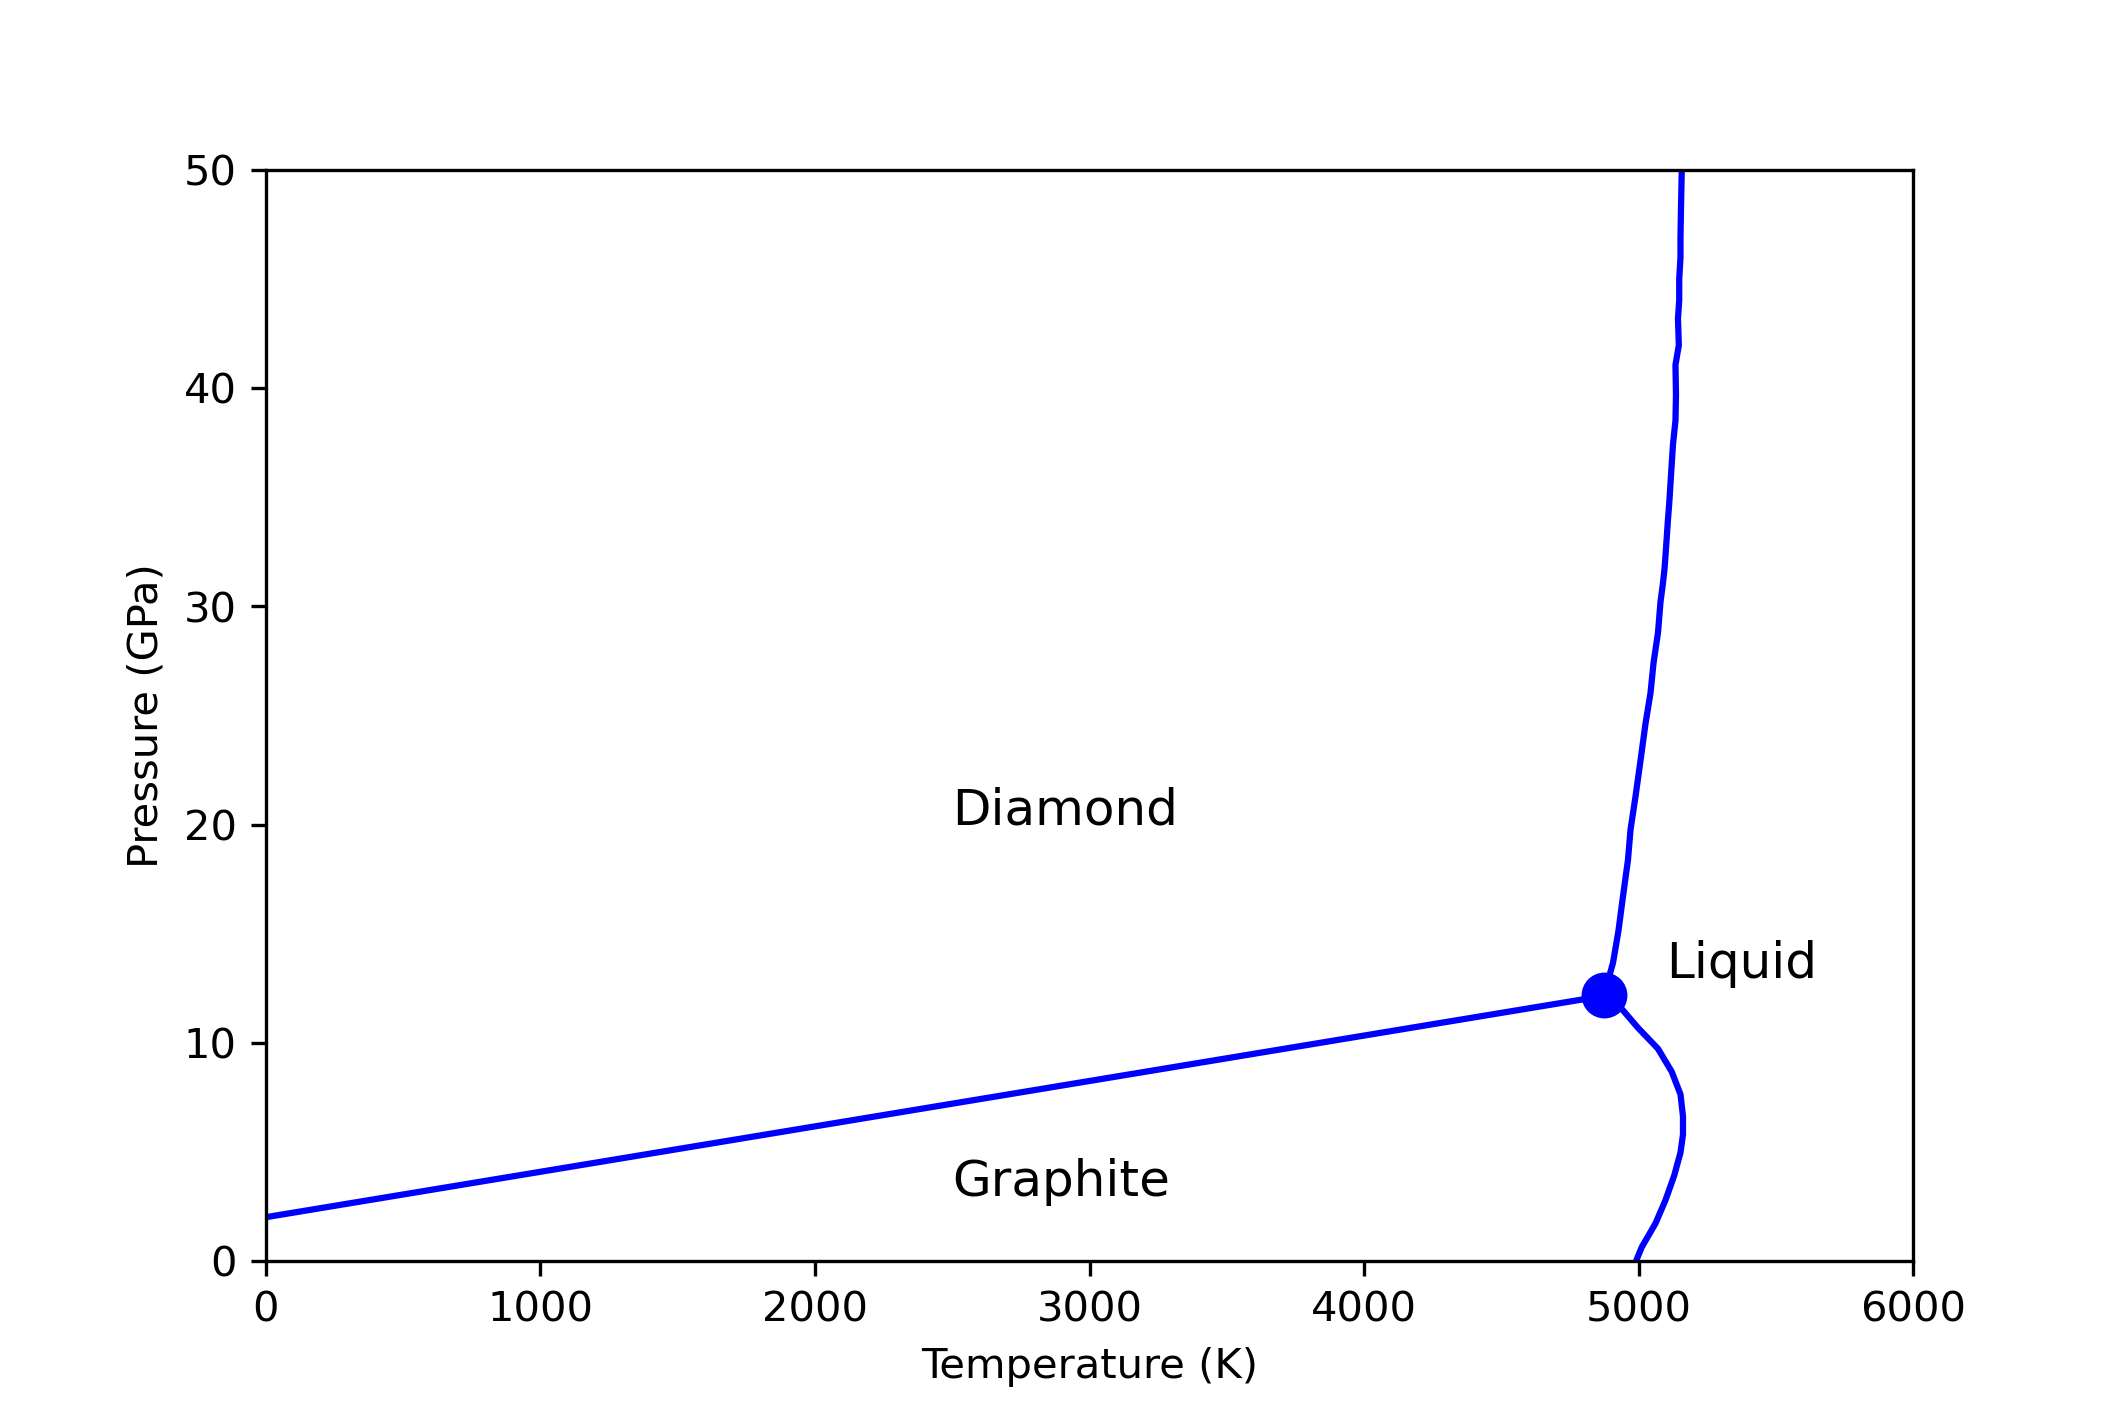
\includegraphics[width=\linewidth]{Chapter2/Figs/Raster/HDphase.png}
	\caption{The simple phase diagram of carbon to 50 \si{\giga\pascal}, which corresponds to approximately a 1500 \si{\kilo\metre} depth within the Earth. Original data sourced from \cite{blank:2018}.}
	\label{fig:phase11}
\end{figure}
The synthesis of diamond has been a focal point in materials science due to the ability to control the supply, quality, size, and dopant levels in synthetic diamonds as compared to their natural counterparts. High-pressure high-temperature (HPHT) and chemical vapour deposition (CVD) methods are the predominant methods employed for the manufacture of both polycrystalline and single-crystal diamonds. Figure \ref{fig:phase11} represents the key phase diagram of interest in the synthesis of diamond. HPHT and CVD synthetic diamonds are cultivated under distinctly different pressure and temperature conditions. The Berman-Simon line \cite{Bundy1961}, which represents the graphite-diamond equilibrium, demarcates the thermodynamically stable region for diamond under HPHT conditions from the graphite-stable region where CVD diamonds are grown \cite{Bovenkerk1993}.

\subsection{HPHT}
\begin{figure}
	\centering
	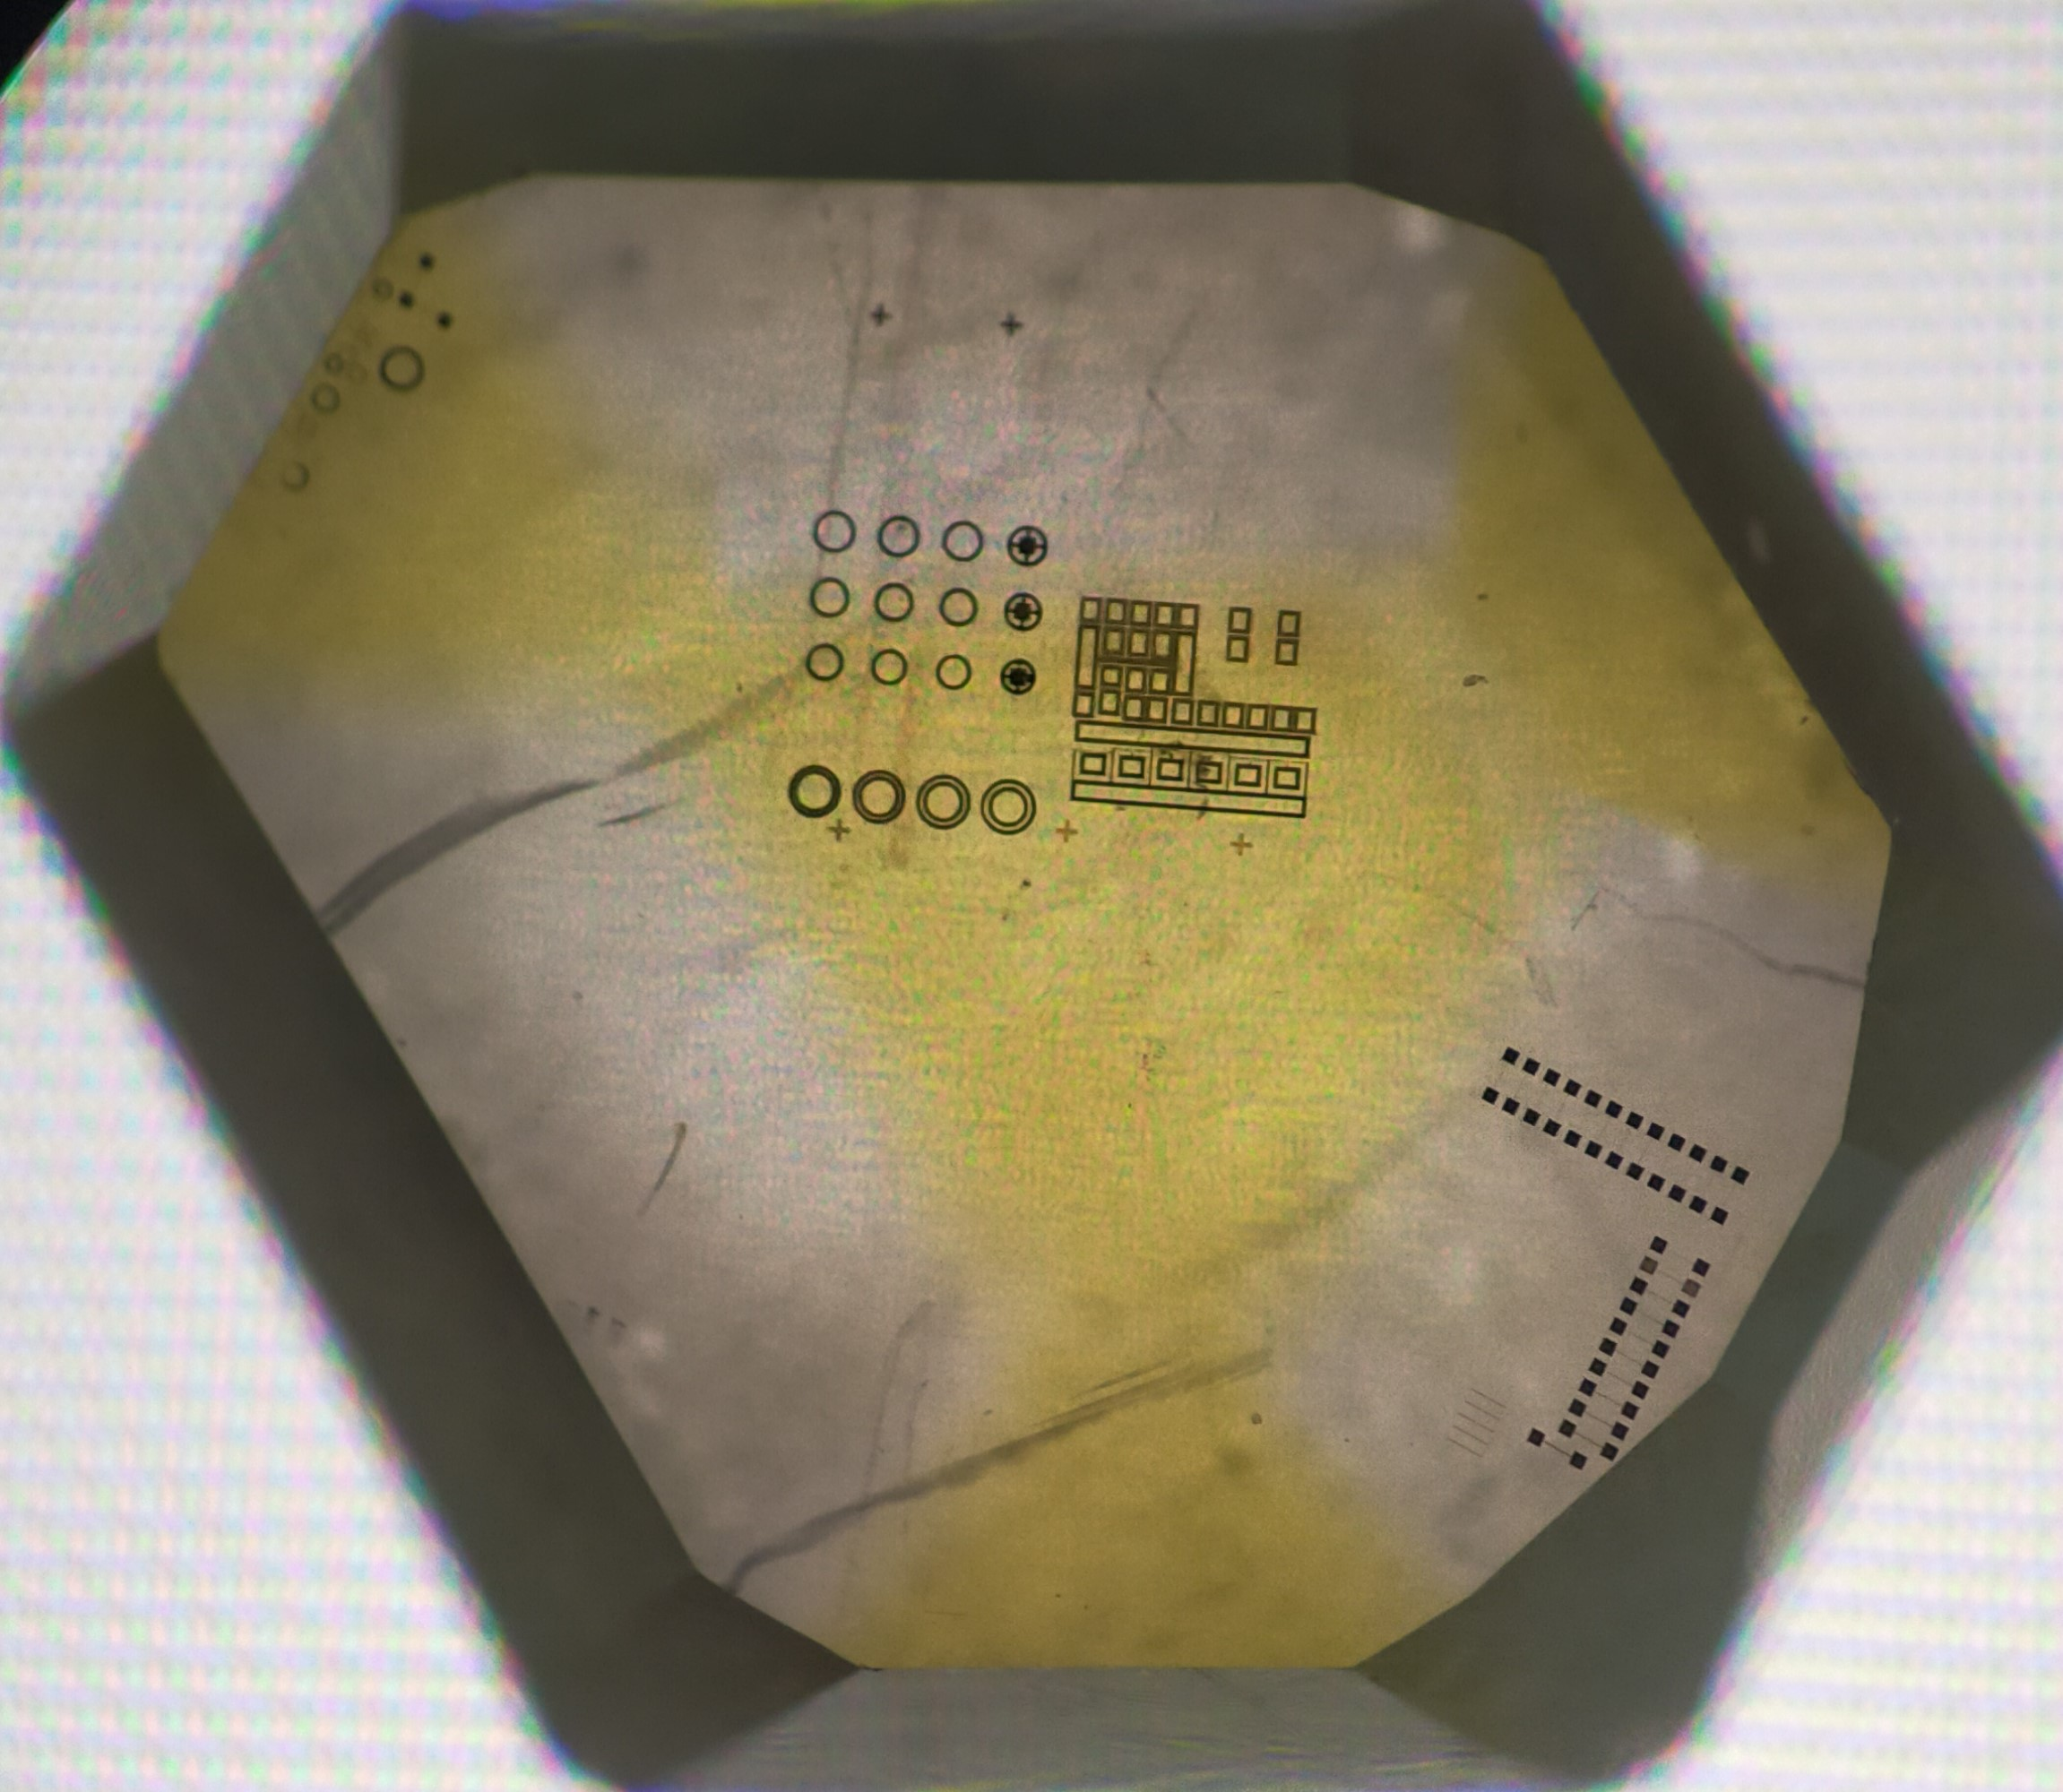
\includegraphics[width=0.5\linewidth]{Chapter7/Figs/Raster/optical back light.jpg}
	\caption{A HPHT substrate used for electrical devices in later chapters.}
	\label{fig:sample1}
\end{figure}
High Pressure High Temperature (HPHT) synthesis replicates the natural conditions under which diamonds form, but allows for enhanced control over the diamonds qualities such as colour and clarity. Early attempts to synthesise diamonds using HPHT began in the 19th century, culminating in the first successful synthesis by General Electric in 1954 \cite{BUNDY1955}. Although high-clarity diamonds are challenging to obtain through HPHT, making this process less desirable for applications requiring optical clarity, advancements have enabled the production of larger, high-quality colourless diamonds for jewellery. One key factor in usage with modern HPHT presses is that of the usage of catalysts, and the careful control of catalyst mixtures \cite{Strong1963}. While it is common for HPHT growth to result in high nitrogen defect concentrations, leading to the characteristic yellow colour as might be seen in figure \ref{fig:sample1}, it is also possible to use nitrogen getters in the catalytic mix, such as Al, Ti, Zr and Mg which will combine with nitrogen atoms to form insoluble nitrates or nitrides, reducing the available nitrogen for incorporation within the growing diamond \cite{Soffner2020}.

\subsection{LMD}
Liquid Metal Diamond (LMD) synthesis represents a novel and promising approach to diamond manufacturing, which operates at significantly lower pressures (1 atm) and moderate temperatures (1025\si{\degreeCelsius}). Unlike traditional methods, LMD uses a liquid metal catalyst at atmospheric conditions composed of elements like gallium, iron, nickel, and silicon to facilitate the growth of diamonds. This method involves catalytic activation of methane and the diffusion of carbon atoms within the liquid metal. Additional hydrogen is also essential, though the exact mechanisms are unclear at this stage. The key physical mechanism of LMD is its ability to supersaturate carbon in the metal, leading to the nucleation and growth of diamond at conditions that are less extreme than those required for either HPHT or CVD \cite{Gong2024}. This method of diamond growth may grow substantially in the near future.

\subsection{CVD}
Chemical Vapour Deposition (CVD) is a highly controlled process used to produce synthetic diamonds by decomposing carbon-rich gases, such as methane, at elevated temperatures (typically 600--1200\si{\degreeCelsius}) in a vacuum chamber. This decomposition is often facilitated by a microwave plasma, although other methods like hot filaments \cite{Kromka2013} and acetylene flames \cite{Garcia1998} are also utilised. The resulting carbon atoms are deposited onto a substrate, forming diamond layers that are particularly useful for applications in electronics and optics due to the versatility in doping and the growth over large areas.

The growth process, significantly influenced by the ratio of hydrogen to methane, is critical in determining the purity, morphology, and overall quality of the diamond films. A plasma generated by microwave power is common in modern CVD setups, but alternative techniques such as hot filaments or blowtorches are also employed. These methods facilitate the dissociation of gas precursors into radicals or ions necessary for diamond growth.

Control over various parameters such as temperature, pressure, gas flow rates, and substrate misorientation is crucial in CVD \cite{Lobaev2019}. Diamond growth via CVD can be categorised into homoepitaxy and heteroepitaxy. Homoepitaxy describes the growth of diamond on a diamond substrate, typically derived from HPHT processes, while heteroepitaxy refers to diamond growth on non-diamond substrates. The latter poses significant challenges due to differences in thermal expansion coefficients and lattice constants, which can lead to defects and dislocations in the diamond film.

CVD technology has evolved since the 1970s, following the pioneering work by Derjaguin et al., who in 1975 demonstrated the feasibility of diamond growth under metastable conditions with cyclic growth and etching processes \cite{derjaguin:1975}. This method was further refined by Spitsyn in 1981 \cite{spitsyn:1981} and Nakazawa in 1987 \cite{nakazawa:1987}, contributing to a deeper understanding of homoepitaxial growth. Concurrently, heteroepitaxial growth has also been explored, with early attempts by Spitsyn in 1981 to grow diamond layers on various substrates such as copper, silicon, and tungsten, among others. These efforts underscored the critical role of atomic hydrogen in suppressing unwanted graphite deposition and enhancing diamond nucleation \cite{kobashi:1988}.

Despite advancements, the heteroepitaxial growth of high-quality, single-crystal CVD diamond remains challenging due to lattice mismatches causing significant strain in the grown layers \cite{Wang2022}. 

\subsection{Doped Diamond}
\subsubsection{Incorporation Efficiency}
\label{subsection:incorporation_efficiency}
In studies examining the growth of n or p-type diamond, it is possible to consider the incorporation efficiency of the dopants involved. First, the density and molar mass of diamond are utilised to calculate the number of carbon atoms present in a cubic centimetre of diamond. With an approximate density of 3.51 \si{\gram\per\centi\metre\cubed} and a molar mass of 12.01 \si{\gram\per\mole}, the number of carbon atoms present can be calculated:
\begin{equation}
    \text{Number of carbon atoms per \si{\centi\metre\cubed}} = \left(\frac{\text{Density}}{\text{Molar mass}}\right)\times N_{A}
    \label{eq:incorporation_efficiency}
\end{equation}
Which results in $\approx1.76\times10^{23}$~\si{\atoms\per\centi\metre\cubed}. For simple reference, it is convenient to consider the magnitudes of phosphorous incorporation and their resulting atomic concentrations. Hence, incorporation efficiencies of 100\%, 10\%, 1\% and 0.1\% are used in the following sections in consideration of the doping concentrations. These efficiencies can then be considered for the various dopant:carbon sources for CVD growth. Naturally, it is unrealistic to consider the extreme cases in which there is no carbon source, but ratios of up to 50\% have been used to grow highly doped diamond films \cite{kato2009, grotjohn2014}. 

Therefore, as in \cite{koizumi1997}, diamond growth where there is a dopant:carbon ratio of 0.1\%, an incorporation ratio of 10\% results in approximately 0.01\% of the dopant being grown into the diamond lattice, corresponding to $0.01\times1.76\times10^{23}=1.76\times10^{19}$~\si{\atoms\per\centi\metre\cubed}. The actual measured concentration of dopant in this example had an incorporation efficiency of around 15\%, with the authors observing $2.5\times10^{19}$ \si{\atoms\per\centi\metre\cubed} of dopant as measured via SIMS analysis. 

\subsection{Phosphorous Doped Diamond}
\subsubsection{Effective Electron Masses}
\label{subsubsec:effective_electron_masses_in_phosphorous_doped_diamond}
Within semiconductors, the effective electron mass is generally determined via the energy-momentum (E-k) relationship for carriers. This describes the interactions of electrons, holes, photons and phonons, and is the basis of semiconductor physics in general. As defined in many semiconductor textbooks, the E-k relationship can be approximated at the band edges (bottom of conduction band $E_{c}$ and top of valence band $E_{v}$) by a quadratic equation \cite{sze2006, Schroder2006-sx, Yu2010, Singleton2001-um}:
\begin{equation}
    E(k) = \frac{\hbar^{2}k^{2}}{2m^{*}}
\end{equation}
where $\hbar$ is the reduced Plank constant, $k$ is the momentum, given as wave vectors and $m^{*}$ is the effective mass. Along a given direction, it is possible to approximate these quadratic curves and estimate the effective mass from the second differential term:
\begin{equation}
    \frac{1}{m_{ij}^{*}} = \frac{1}{\hbar^{2}}\frac{\partial^{2} E(k)}{\partial k_{i}\partial k_{j}}
\end{equation}
where the indices i, j are used to indicate the tensorial components of effective mass in differing momentum space directions. The conduction band is made up of a number of sub-bands, with the bottom of the conduction band appearing either at the centre (given by the standard Wigner-Seitz cell symmetry notation of $\Gamma$) or at another position in k-space. Similarly, the valence band is made up of a number of sub-bands, which may or may not line up with the bottom of the conduction band. Semiconductors in which the bandgap is aligned are known as direct-bandgap semiconductors, such as InAs, GaN and GaAs. These semiconductors are of particular interest for applications involving radiative emission, as the emission of light in direct bandgap semiconductors has a significantly greater quantum efficiency due to the lack of change in momentum required (requiring phonon interactions). Indirect bandgaps in which a change in momentum space is necessary for electronic transitions across the bandgap are seen in Si, Ge and also C - that of the sp$^{3}$ bonded diamond crystal lattice of carbon. While it is common practice to refer to semiconductors by their shorthand elemental composition, this does not work very well with that of carbon due to the quantity, diversity and colossal range of carbon allotropes.

\begin{figure}[H]
    \centering
    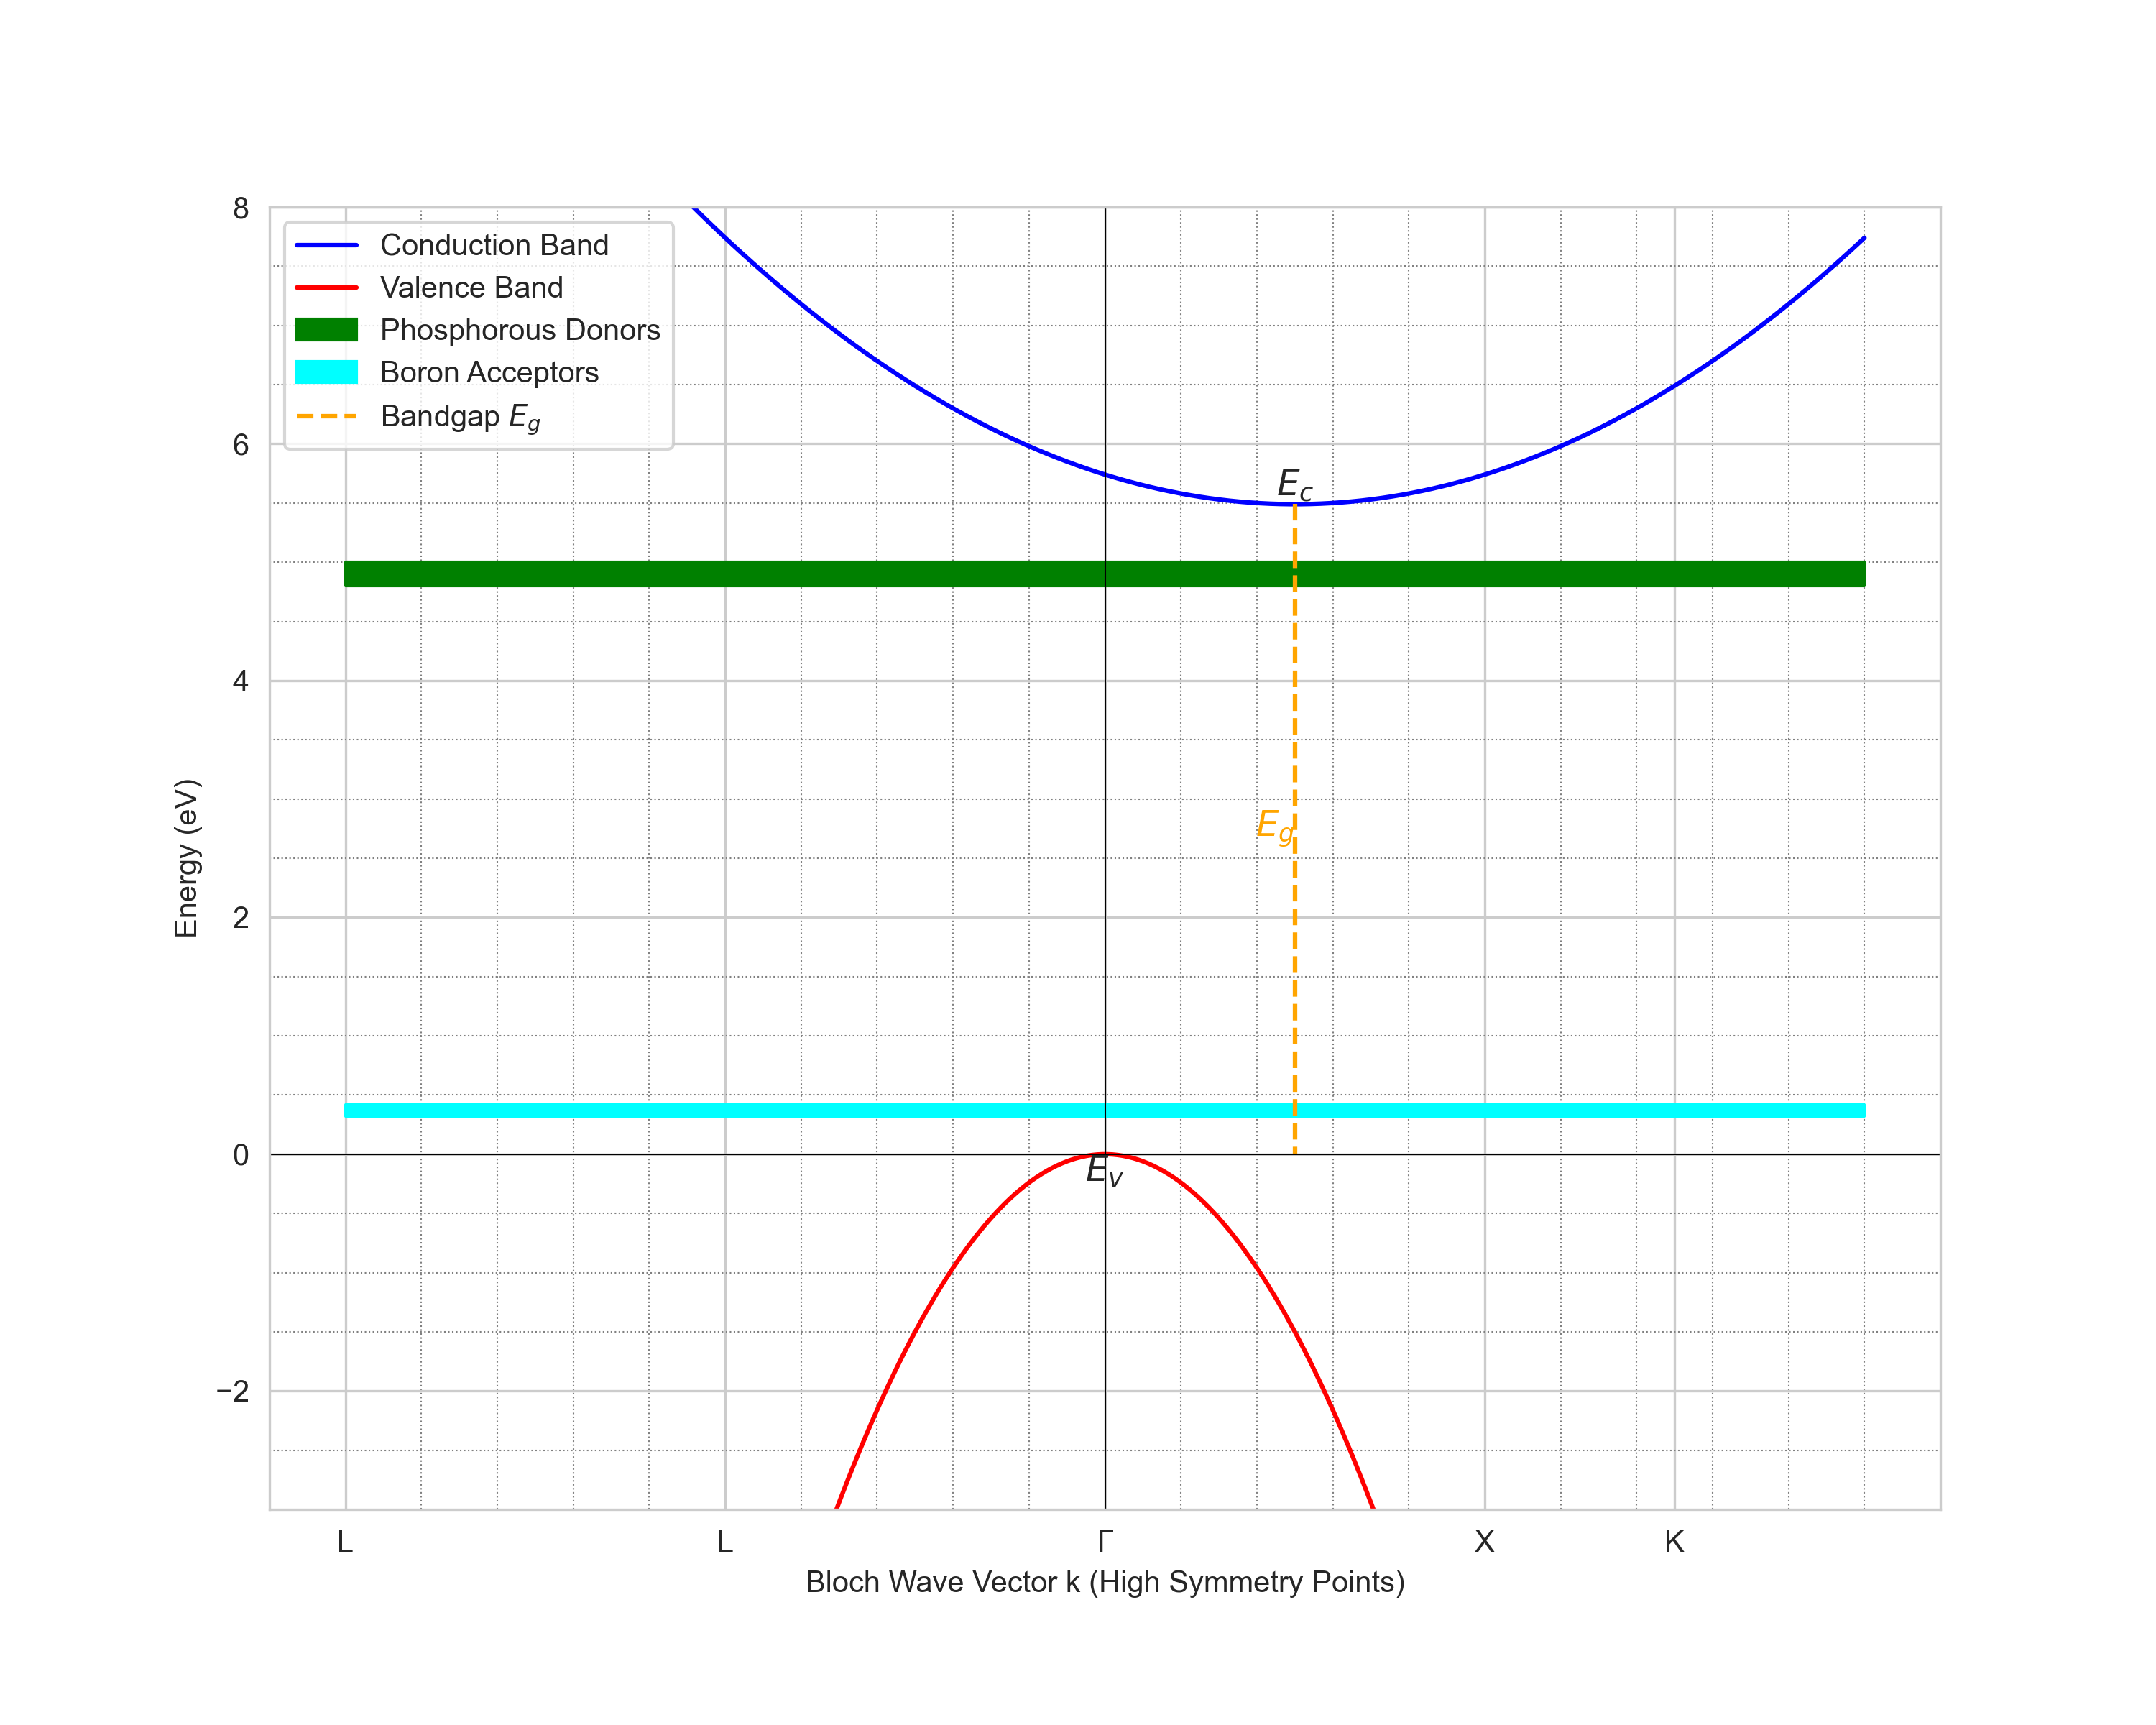
\includegraphics[width=\textwidth]{Chapter2/Figs/Raster/python_band_structure.png}
    \caption{An approximate depiction of the parabolas responsible for diamond's electronic band structure. Loosely based on the full electronic structure as depicted in \cite{Willatzen1994}, including highly simplified defect states of phosphorous and boron.}
    \label{fig:band_parabolas}
\end{figure}

Figure \ref{fig:band_parabolas} shows a simplified parabola representation of of diamond. Shown is an indirect bandgap, which is measured at low temperatures approaching 0~\si{\kelvin} to be 5.49~\si{\electronvolt} via transmission/absorption spectra \cite{clark1964, Mildren2013} and density of states calculations \cite{Sellam23}. For a full review of diamond dopant species and surface terminations on the electronic properties, such as the bandgap, see the work by Prof. K. Larsson \cite{Larsson2020}.

The determination of effective carrier masses has been obtained in several ways throughout the literature. For the work described in following chapters, the effective mass of electrons within highly phosphorous doped diamond is of particular interest, but for ultra-pure intrinsic diamond, it has been experimentally observed via time-resolved cyclotron resonance that the transverse and longitudinal electron masses are $0.280m_{0}$ and $1.56m_{0}$ respectively \cite{Naka2013}. These values represent what is currently believed to be the top-end limit of high velocity carriers within intrinsic diamond. A more relevant example of experimental measurements is that of Gheeraert et al. \cite{Gheeraert2001} who used infrared absorption to observe the electronic transitions for phosphorous donors and hence determine the effective mass within electronically active, doped diamond films. In this work, the effective masses are determined to be $m_{\perp}=0.306m_{0}$ and $m_{\parallel} = 1.81m_{0}$. These are the values that are widely used as reference values for phosphorous doped diamond \cite{Pernot2006, Pernot2008}, and will hence be used in this work as a reference point also. These values can be contrasted to theoretically based work using a linear muffin-tin-orbital local density approximation for intrinsic diamond by Willatzen et al. who gave values of $m_{\perp}=0.341m_{0}$ and $m_{\parallel}=1.5m_{0}$. A final comparison is measured via a Monte Carlo analysis of electron drift velocity \cite{Nava1980} by Nava et al. This is one of the earliest works in studying this property via Hall effect measurements, giving values of $m_{\perp}=0.36m_{0}$ and $m_{\parallel}=1.4m_{0}$ for intrinsic diamond.

\section{Graphitisation of Diamond} % Chapter title

\label{sec:laser} % For referencing the chapter elsewhere, use \autoref{ch:examples} 

%----------------------------------------------------------------------------------------

The roots of laser graphitisation in diamond can be traced back to 1996, with a seminal paper by Davies et al. demonstrating that the usage of tightly focused femtosecond laser pulses could be used to permanently modify the optical properties of a small volume within the transparent substrate \cite{davies:1996}. With careful tuning of the irradiation conditions, it is possible to induce a localised refractive index increase within the focal volume, allowing for the writing of optical waveguides with only a translation of the substrate. 

The advantages of this technique can also be seen through the lens of diamond device processing and graphitisation rather than the tuning of optical properties, though a significant portion of the current industrial applications for laser graphitisation within diamond are in writing serial numbers and other optical markers for jewellers to identify lab-grown diamond:

\begin{itemize}
	\item Laser fabrication is a direct, mask-less technique. Without the need for complex clean room facilities it is possible to create surface tracks or buried wires within the diamond. This allows for the rapid prototyping and refinement of a small number of devices, without the added need of dedicated photolithographic masks.
	\item This technique is highly flexible, as different irradiation parameters such as wavelength, pulse energy, translation speed, focusing conditions and repetition rate can be used to calibrate the laser for different materials like silicon carbide, diamond and other crystal structures. This also allows for more specific control over the graphitic content which is formed within the diamond substrate, with differing conductivities for various sp$^{2}$ and sp$^{3}$ content in the formed wires.
	\item With the usage of adaptive optics it is possible to create fully three-dimensional graphitic wires within the diamond substrate, of various thicknesses and conductivities at arbitrary depths. The degrees of freedom offered by this technique allow for geometries that are impossible or highly difficult with standard fabrication techniques, which may be an important factor in the design and manufacturing of certain device structures. 
\end{itemize}

\clearpage
%----------------------------------------------------------------------------------------

\begin{figure}
	\centering
	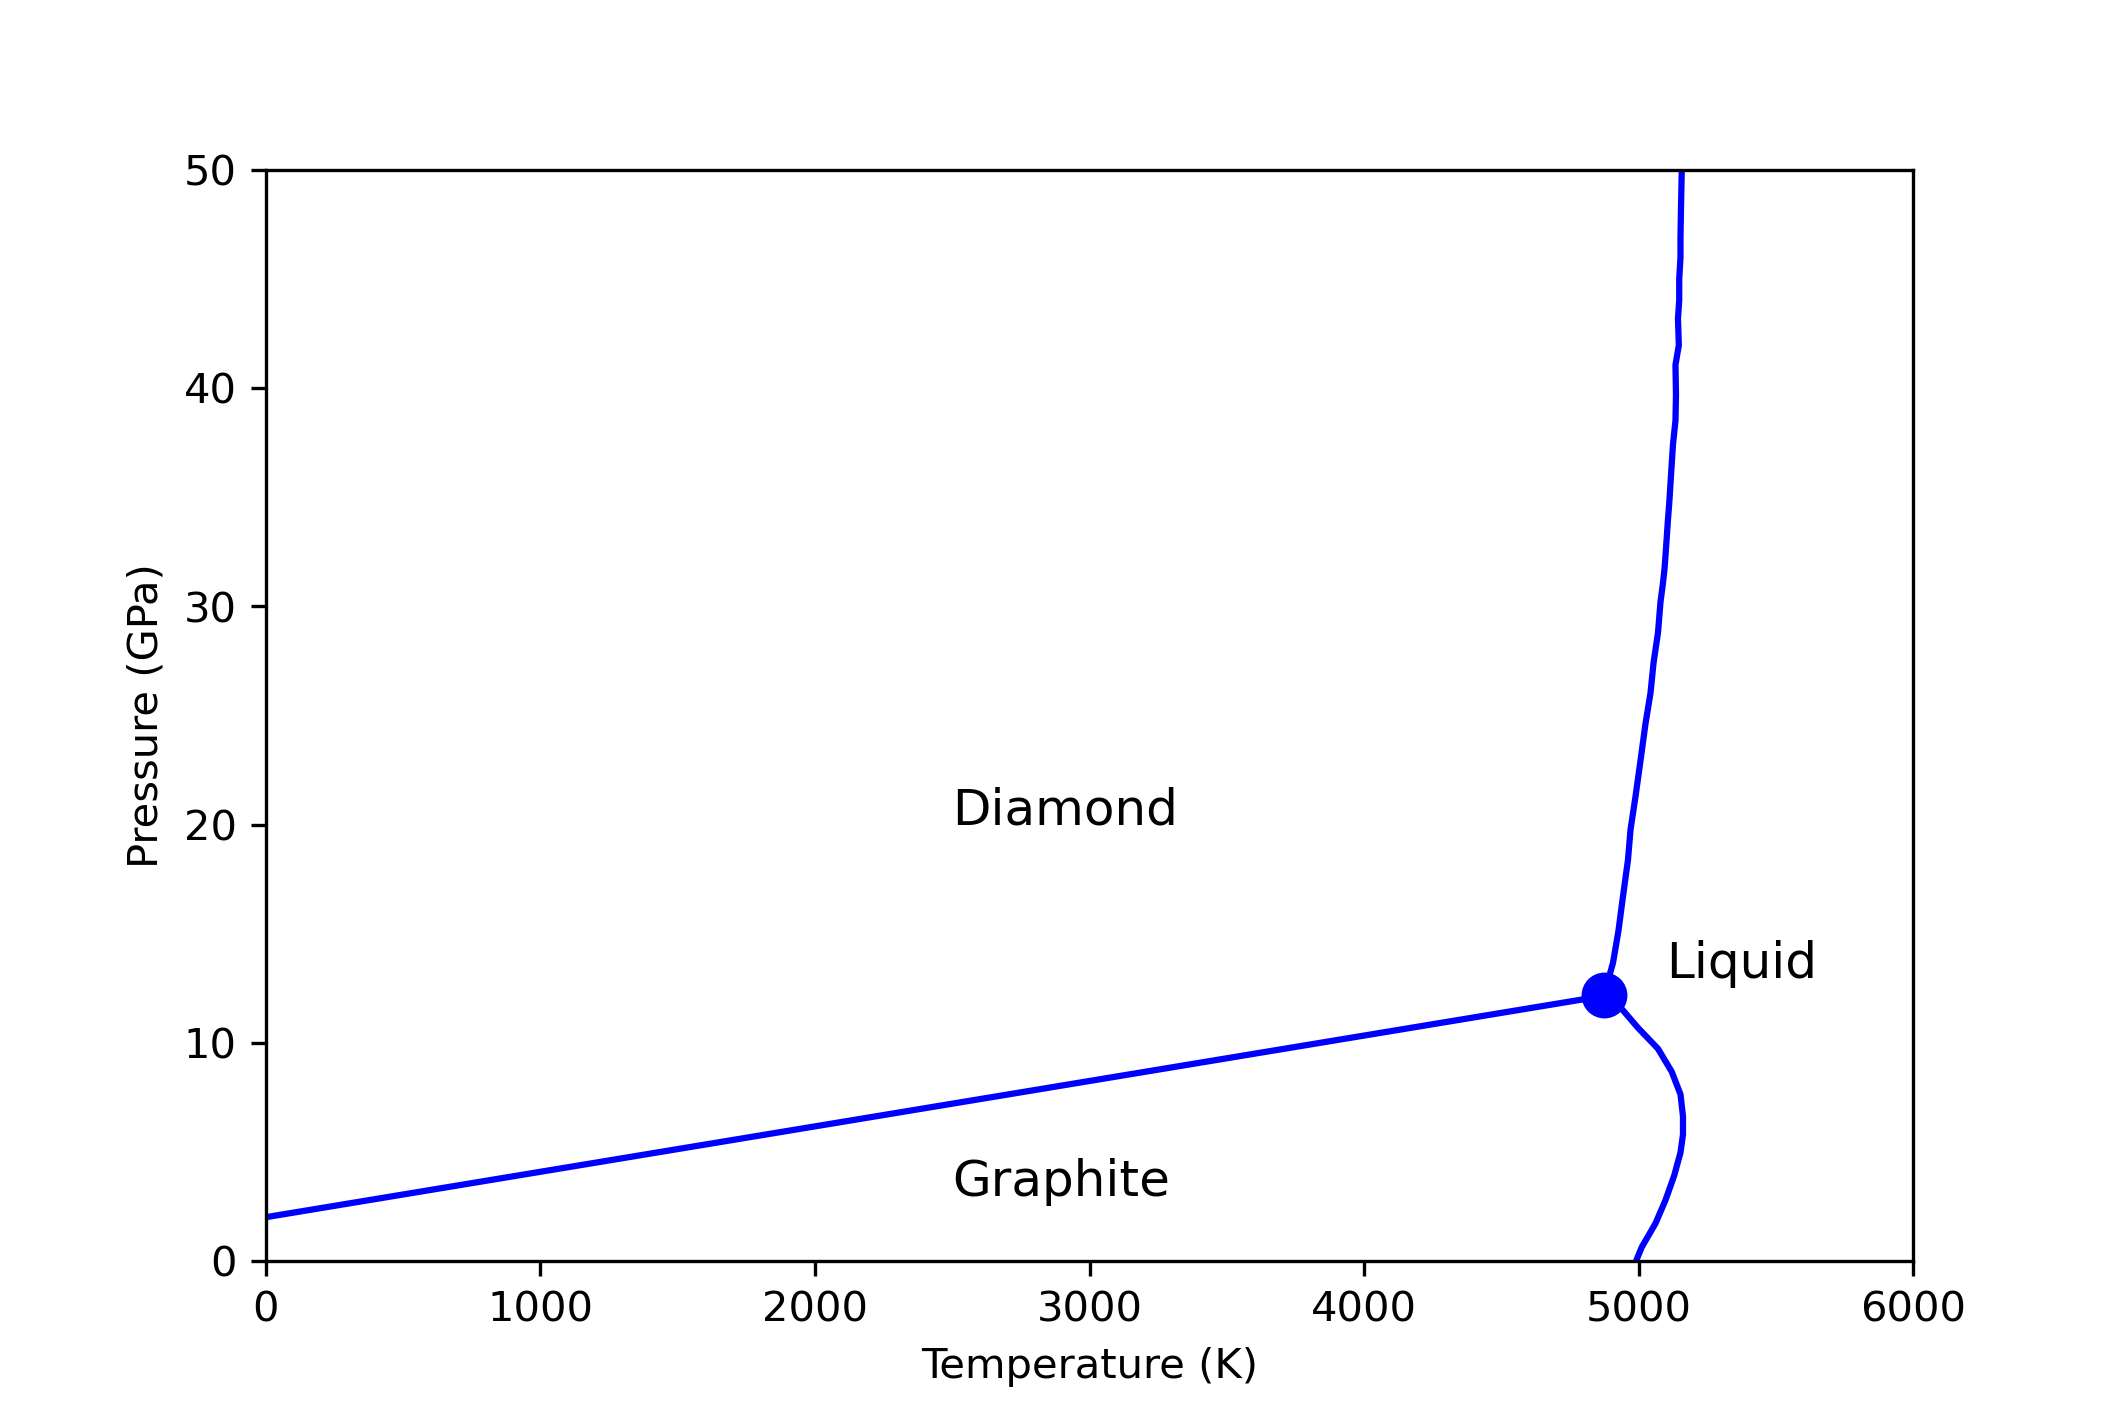
\includegraphics[width=\linewidth]{Chapter2/Figs/Raster/HDphase.png}
	\caption{The simple phase diagram of carbon to 50 \si{\giga\pascal}, which corresponds to approximately a 1500 \si{\kilo\metre} depth within the Earth. Original data sourced from \cite{blank:2018}.}
	\label{fig:phase}
\end{figure}

The fundamental process of writing graphitic regions within diamond is governed by the crystal structure meta-stability. At room temperature and under atmospheric pressure the stable phase of carbon is that of graphite, as shown in figure \ref{fig:phase}, hence when the diamond lattice damage density exceeds a critical value, it will form graphite. This can also be viewed as a sufficient number of diamond sp$^{3}$ bonds being broken, then reforming into the stable graphitic phase with sp$^{2}$ bonds. One simple way to cause this damage to a diamond lattice is to essentially burn it, or otherwise raise the temperature of the sample. A diamond lattice will tend to rearrange globally when heated to $T_{G} \approx 2000$ \si{\kelvin}, which is called the process of thermal graphitisation \cite{davies:1972}. However, it has been observed that in cases where a laser pulse does not generate this critical temperature, graphitisation may still occur. 

\subsection{Ion Implantation}
Another way to break the diamond sp$^{3}$ bonds is to bombard the diamond lattice with ions of a sufficiently high kinetic energy to also break the sp$^{3}$ bonds. Ion implantation was first investigated in the 70s by Vavilov et al \cite{vavilov:1973}, and resulted in a series of studies examining the electrical properties of the resultant amorphous carbon. Hauser et al. demonstrated the similarities of sputtered graphite to that of the ion implanted diamond, with a high conductivity of $\approx10^{-2}$ \si{\per\ohm\per\centi\metre} and also concluded that the resulting hardness of the implanted regions was an intermediate between that of silicon and diamond \cite{hauser:1976,hauser:1977}. With the proper combinations of implanting ions, ion energies, dosages and post implantation annealing, diamond based heterostructure can be formed which have layers of insulating, semi-conducting, luminescent and fully conductive regions \cite{gippius:1999,prins:1983,prins:1985}. 

One more specific case occurs in the case of implanting boron ions in polycrystalline diamond, where a "percolative threshold" fluence exists at which a conductive path of sp$^{3}$ bonded defects is formed in the diamond structure and a variable range hopping conduction mechanism is introduced. At a higher "amorphisation threshold", sp$^{2}$ bonded defects are formed, leading to permanent graphitisation in the implanted areas after annealing \cite{fontaine:1995}.

\subsection{Laser Graphitisation}
In the case of laser graphitisation, the mechanism of localised heating through the non-linear absorption of laser pulses requires some clarification, especially since diamond is generally regarded as a "thermal short" with its thermal conductivity of up to 2200-2500 \si{\watt\per\metre\per\kelvin} \cite{graebner:1995}. As presented in an article by Sundaram and Mazur in 2002, while intense laser pulses from a nanosecond pulsed laser within silicon is a thermally driven process, experimentally observed ultrashort femtosecond laser pulse effects cannot be explained with merely a thermal process \cite{sundaram:2002}. Instead, the femtosecond pulses drive a large fraction of the valence electrons ($>10\%$) into the conduction band, modifying the inter-atomic forces and destabilising the crystal lattice. A model presented by Kononenko et al. in 2015 relies primarily upon the expansion of graphitic inclusions through so called photographitisation, and argues that the laser induced direct creation of graphitic nucleation sites within diamond is unlikely \cite{kononenko:2015}. Instead, graphite inclusion defects within the diamond structure are the source, with inclusions forming the seeds of growing and overlapping graphitic regions. This growth of inclusions is then a two step process, with a distinct mechanism for each stage. Similar work presented by Bennington et al. in 2009 on single crystal (111) oriented HPHT diamonds concurs with this model, observing that the generated graphite was likely seeded by defects within the crystal lattice \cite{bennington:2009}.

\subsubsection{Photographitisation}
Under femtosecond irradiation, it has been observed that the transition from diamond to graphite is not one driven by a thermal process, but instead it is one driven by an electron-hole plasma that is generated by the laser. Pulsed X-ray diffraction experiments in germanium, silicon, GaAs and InSb observed this same process in 1999 and 2001 with the laser-induced promotion of a large fraction of valence electrons (more than $10$\%) and with a low "melting time" on the order of femtoseconds \cite{siders:1999,rousse:2001}. Once excited, these electrons strongly interact with one another and reach thermal equilibrium in under 10 \si{\femto\second} \cite{elsaesser:1991}.
Through the process of photoionisation, light is absorbed by the substrate and photon energy promotes electrons from bonding orbitals in the valence band to the conduction band, in unbound or even antibonding states. This absorption within diamond is a multiphoton process, depending upon the lasing wavelength. For $800$ \si{\nano\metre}, there is a four or five photon transition, while $400\text{ and }266$ \si{\nano\metre} wavelengths have an indirect and two photon transition respectively \cite{preuss:1995}. The direct band gap in intrinsic diamond for these transitions is $7.3$ \si{\electronvolt}. However, the presence of substitutional nitrogen or phosphorous will introduce donor like centres with a thermal ionisation energy of $1.7$ \si{\electronvolt} and $0.6$ \si{\electronvolt} respectively, complicating the band structure. The electron-hole density within diamond when illuminated by Kononenko et al. with a \ce{TiAl2O3} laser of wavelength $800$ \si{\nano\metre} at fluencies of under $10$ \si{\joule\per\centi\metre\squared} reached up to $10^{21}$ \si{\per\centi\metre\cubed}. The experimental data from this work is plotted in figure \ref{fig:electronholes}.

\begin{figure}
	\centering
	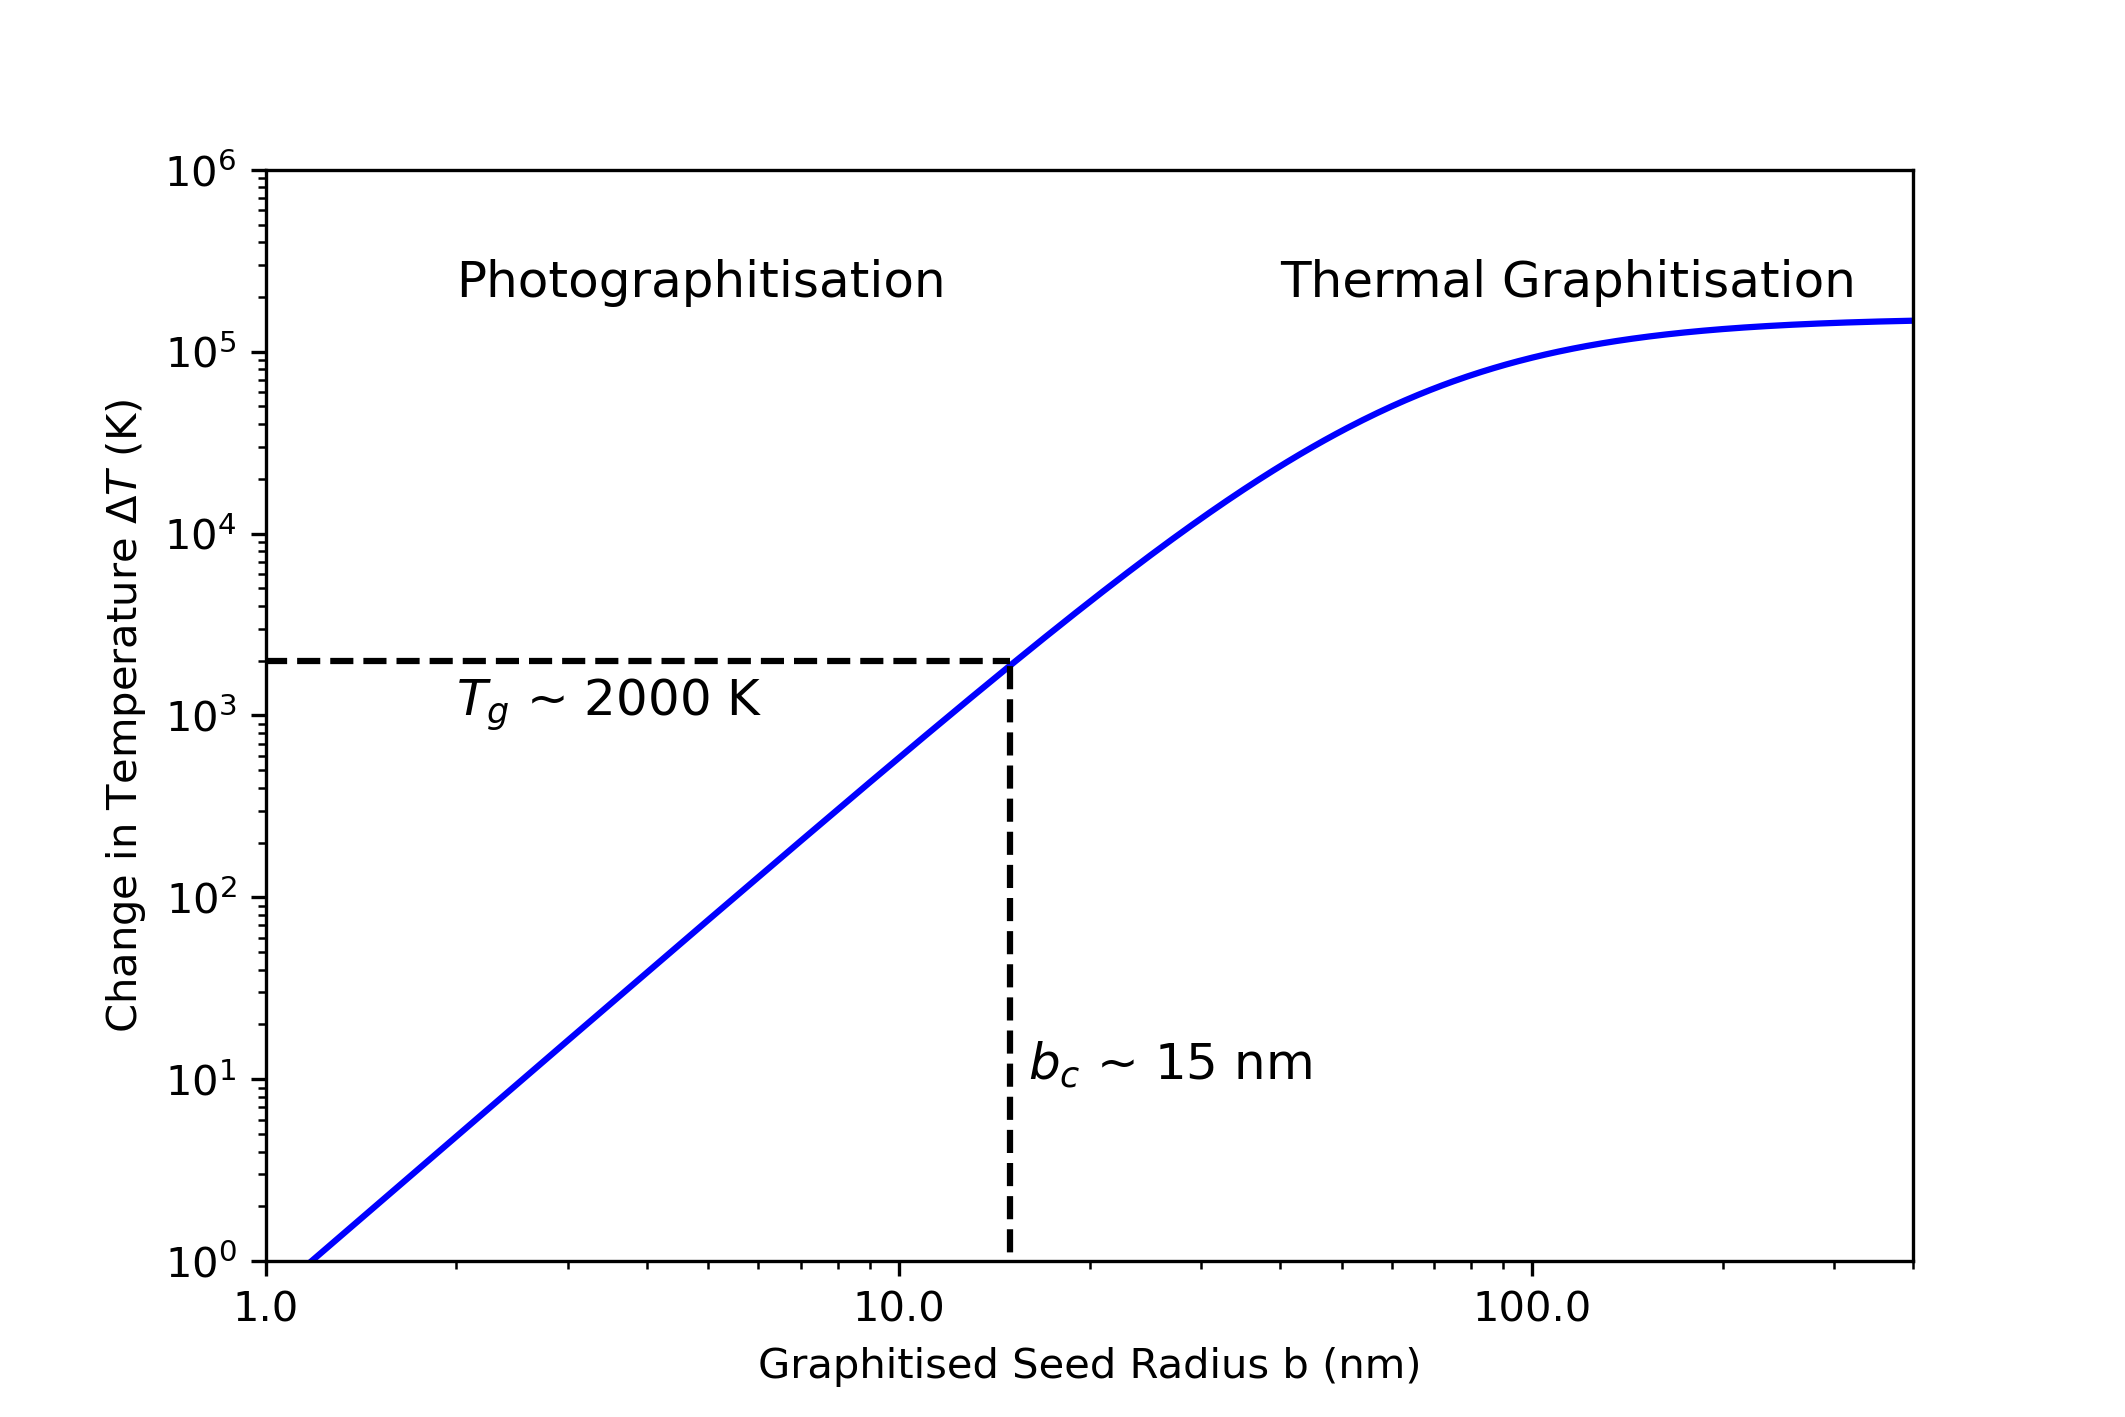
\includegraphics[width=\linewidth]{Chapter2/Figs/Raster/HDelectronholes.png}
	\caption{The concentration of electron hole pairs in single crystal diamond just below the crystal surface, as measured by Kononenko et al \cite{kononenko:2014}.}
	\label{fig:electronholes}
\end{figure}

In the case of a perfect diamond lattice, these generated electron hole pairs would eventually relax and reform the \ce{C-C} bonds of sp$^{3}$ orbitals. The diamond lattice is highly rigid, which prevents the deformation of bonds via electron hole pairs in contrast to other wide band gap semiconductors \cite{martin:1997}. However, when these electron hole pairs are generated close to the edge of a graphite inclusion or other such graphitic region, then the chemical bonds making up the diamond lattice experience a significant distortion due to local Coulomb forces. Hence when there is a significant density of electron hole pairs, the \ce{C-C} bonds at the interface of diamond and graphite have a chance to change in hybridisation from sp$^{3}$ to sp$^{2}$ orbitals, permanently breaking the diamond lattice and expanding the graphitic region. The exact ratio of sp$^{2}$/sp$^{3}$ within an amorphous carbon structure such as that formed under photographitisation may vary in regions, but areas of less graphitic content may have a ratio approaching 3 based on previous XPS/XAES measurements of amorphous carbon as formed with ion bombardment \cite{lascovich:1991}. Under subsequent pulses of laser irradiation, this process will slowly expand the graphitic inclusion, layer by layer.

\subsubsection{Density Functional Theory}
Through the usage of DFT, atomistic calculations examining the transition from diamond to graphite have estimated that the graphitisation due to photoionisation will complete within $100$ \si{\femto\second} \cite{jeschke:1999} to $200$ \si{\femto\second} \cite{wang:2000}. In particular, the work by Wang et al in 2000 examined the particular case of laser induced graphitisation on the (111) surface. This is particularly relevant for devices written on phosphorous doped, n-type diamond, as the (111) surface provides the highest dopant concentration and also most active carrier concentration when compared to other growth facets. Their conclusions can be summarised as:

\begin{itemize}
	\item When the overall diamond temperature reaches 2700 \si{\kelvin} the surface will rapidly graphitise.
	\item Graphitisation occurs vertically for the simulations of longer pulse (nanosecond) durations, with graphite-like regions penetrating down through the surface layers into the bulk.
	\item Graphite sheets are formed in the case of femtosecond pulse durations, with a reduced time for complete graphitisation at higher effective electron temperatures.
	\item The energy barrier to graphitisation is lower in the case of higher electron temperatures, also corresponding to a reduced time required for complete graphitisation.
\end{itemize}

More recent studies examining the stability of diamond and graphite bonds with larger supercells provide further confirmation of the energy barrier between the two carbon hybridisations \cite{popov:2019,grochala:2014}. A first-principle study by F. Mauri in 1995 explored the electron lattice interactions, concluding that valence excitons are highly likely to bind together when in a high density electron-hole plasma \cite{mauri:1995}. Self-trapping does not occur in the case of isolated valence excitons, but it is predicted that self trapping should occur with valence biexcitons. This biexciton trapping will cause a distortion, involving the breaking of a bond perpendicular to the (111) direction. As graphite is semi-metallic in nature, electron-hole pairs migrating from the excited diamond regions to that of a graphite seed will rapidly multiply through impact ionisation. Impact will also reduce their energy below the diamond band gap, trapping such pairs and collecting them within the graphitic region. Graphite's $\pi$ orbitals are able to hold a large number of electron-hole pairs without changing the covalent bond network, lending a greater stability to the graphite region than the diamond in conditions of high electron-hole pairs in addition to the refractory nature of graphite \cite{bennington:2009}.

\begin{figure}
	\centering
	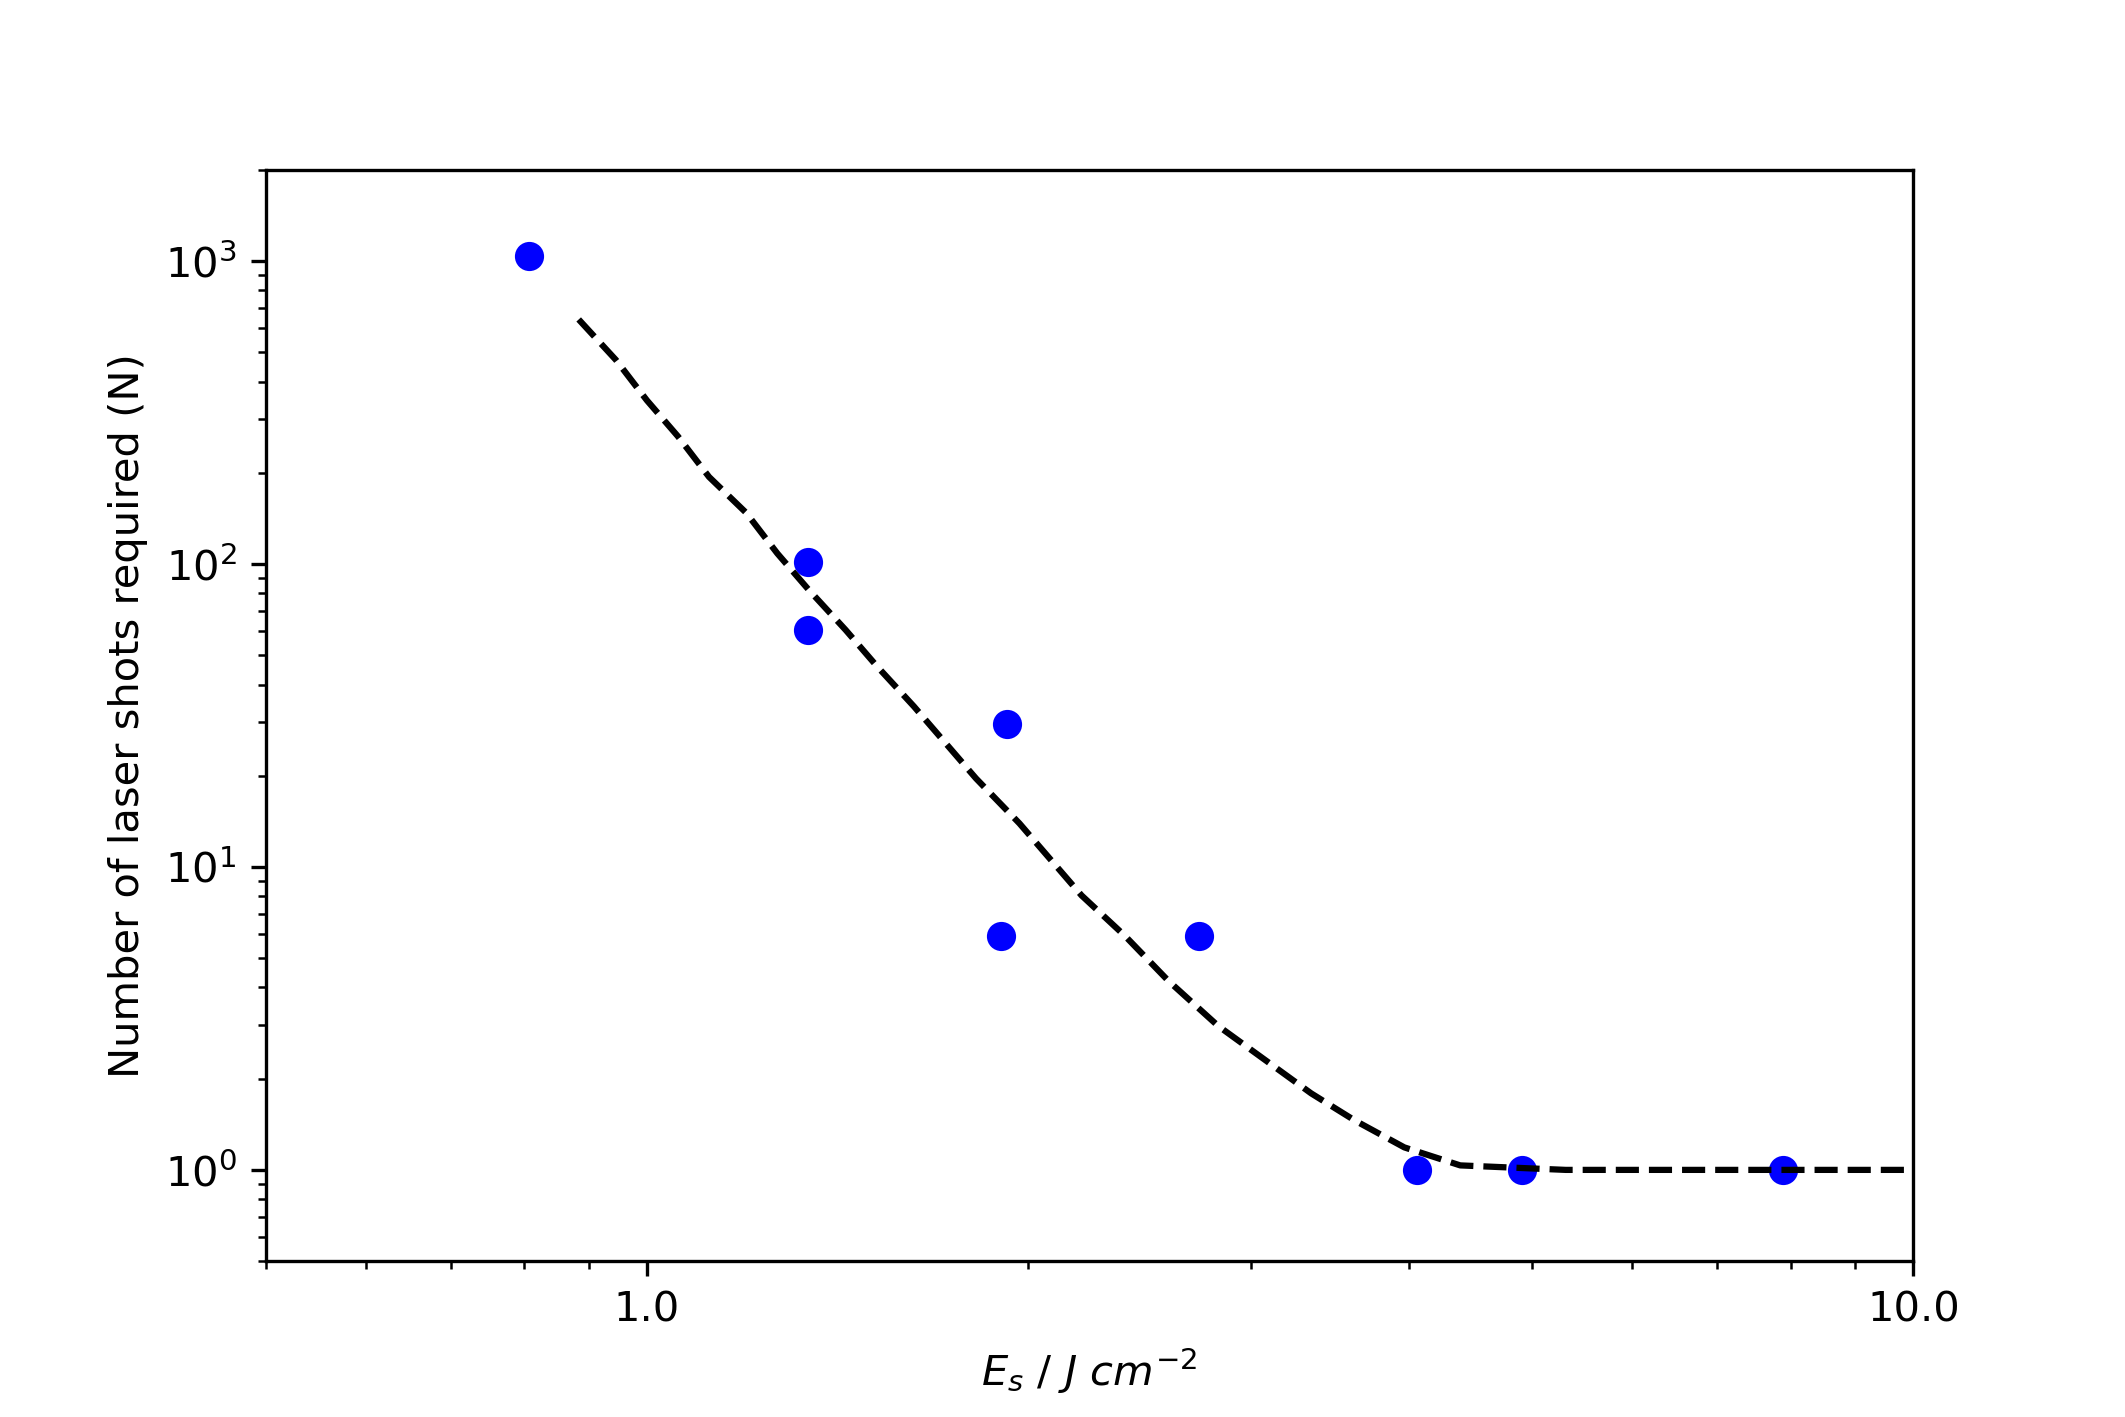
\includegraphics[width=\linewidth]{Chapter2/Figs/Raster/HDfluencevsshots.png}
	\caption{The number of laser shots required for visible damage of the diamond surface as a function of laser fluence, as measured by Kononenko et al \cite{kononenko:2008}.}
	\label{fig:fluencevsshots}
\end{figure}

\subsubsection{Thermal Graphitisation}
\label{subsubsec:thermal_graphitisation}
As these graphite seeds grow due to the photostimulated lattice rearrangement of carbon atoms adjacent to the graphite, the amount of light that is absorbed due to the change in the optical properties will increase. Also, when stimulated by light, the electron subsystem of graphite will take longer to relax than its sp$^{3}$ counterpart from the excited $\pi$-band electron population. This effect slows the heating of graphitic regions on a scale of $\tau_{e-ph}\approx1$ \si{\pico\second}, where $\tau_{e-ph}$ is the electron-phonon thermalisation \cite{seibert:1990}. Diamond has a remarkably high thermal diffusivity of $\chi_{d}\approx10$ \si{\centi\metre\squared\per\second} \cite{tokmakoff:1993}. This is high enough that the process of thermalisation can overlap in time with the heat spreading from graphite seeds into the diamond lattice. Hence, the temperature of these diamond seeds as induced by laser stimulation will strongly depend upon the seed size, which can be expressed in the following way:

\begin{equation}
\Delta T \approx\sigma_{a}F/l_{D}^{3}/c_{d}
\label{eq:deltaT}
\end{equation}
\begin{equation}
\sigma_{a} \approx \frac{2\pi}{\lambda}Im\left(4\pi b^{3}\frac{\epsilon_{g}-\epsilon_{d}}{\epsilon_{g}+2\epsilon_{d}}\right)
\label{eq:sigma laser}
\end{equation}
\begin{equation}
l_{D} = \left(4\chi_{d}\tau_{e-ph}+b^{2}\right)^{1/2}
\label{eq:ld laser}
\end{equation}

Where $\sigma_{a}$ is the absorption cross section, $\epsilon_{g}=6.0825+10.673i$ \cite{djurisic:1999} is the permittivity of graphite and $\epsilon_{d}=5.76$ \cite{phillip:1964} is the permittivity of diamond, $F$ is the laser fluence, $b$ is the graphite seed radius and $c_{d}=1.75$ \si{\joule\per\centi\metre\cubed\per\kelvin} is the specific heat capacity of diamond \cite{prelas:1997}. The energy absorbed by the graphite seed will dissipate in a volume $l_{D}^{3}$, defined by the current radius of the seed and the heat diffusion length within diamond. Heat diffusion length is defined by the thermalisation time of electron-phonons  $\tau_{e-ph}\approx1$ \si{\pico\second}. $\Delta T\left(b\right)$ as calculated with equations \ref{eq:deltaT}, \ref{eq:sigma laser}, \ref{eq:ld laser} at a fluence of $0.75$, $1.5$ and $3$ \si{\joule\per\centi\metre\squared} and $\tau_{e-ph}=1$ \si{\pico\second} is depicted in figure \ref{fig:laser-heating}.

\begin{figure}
	\centering
	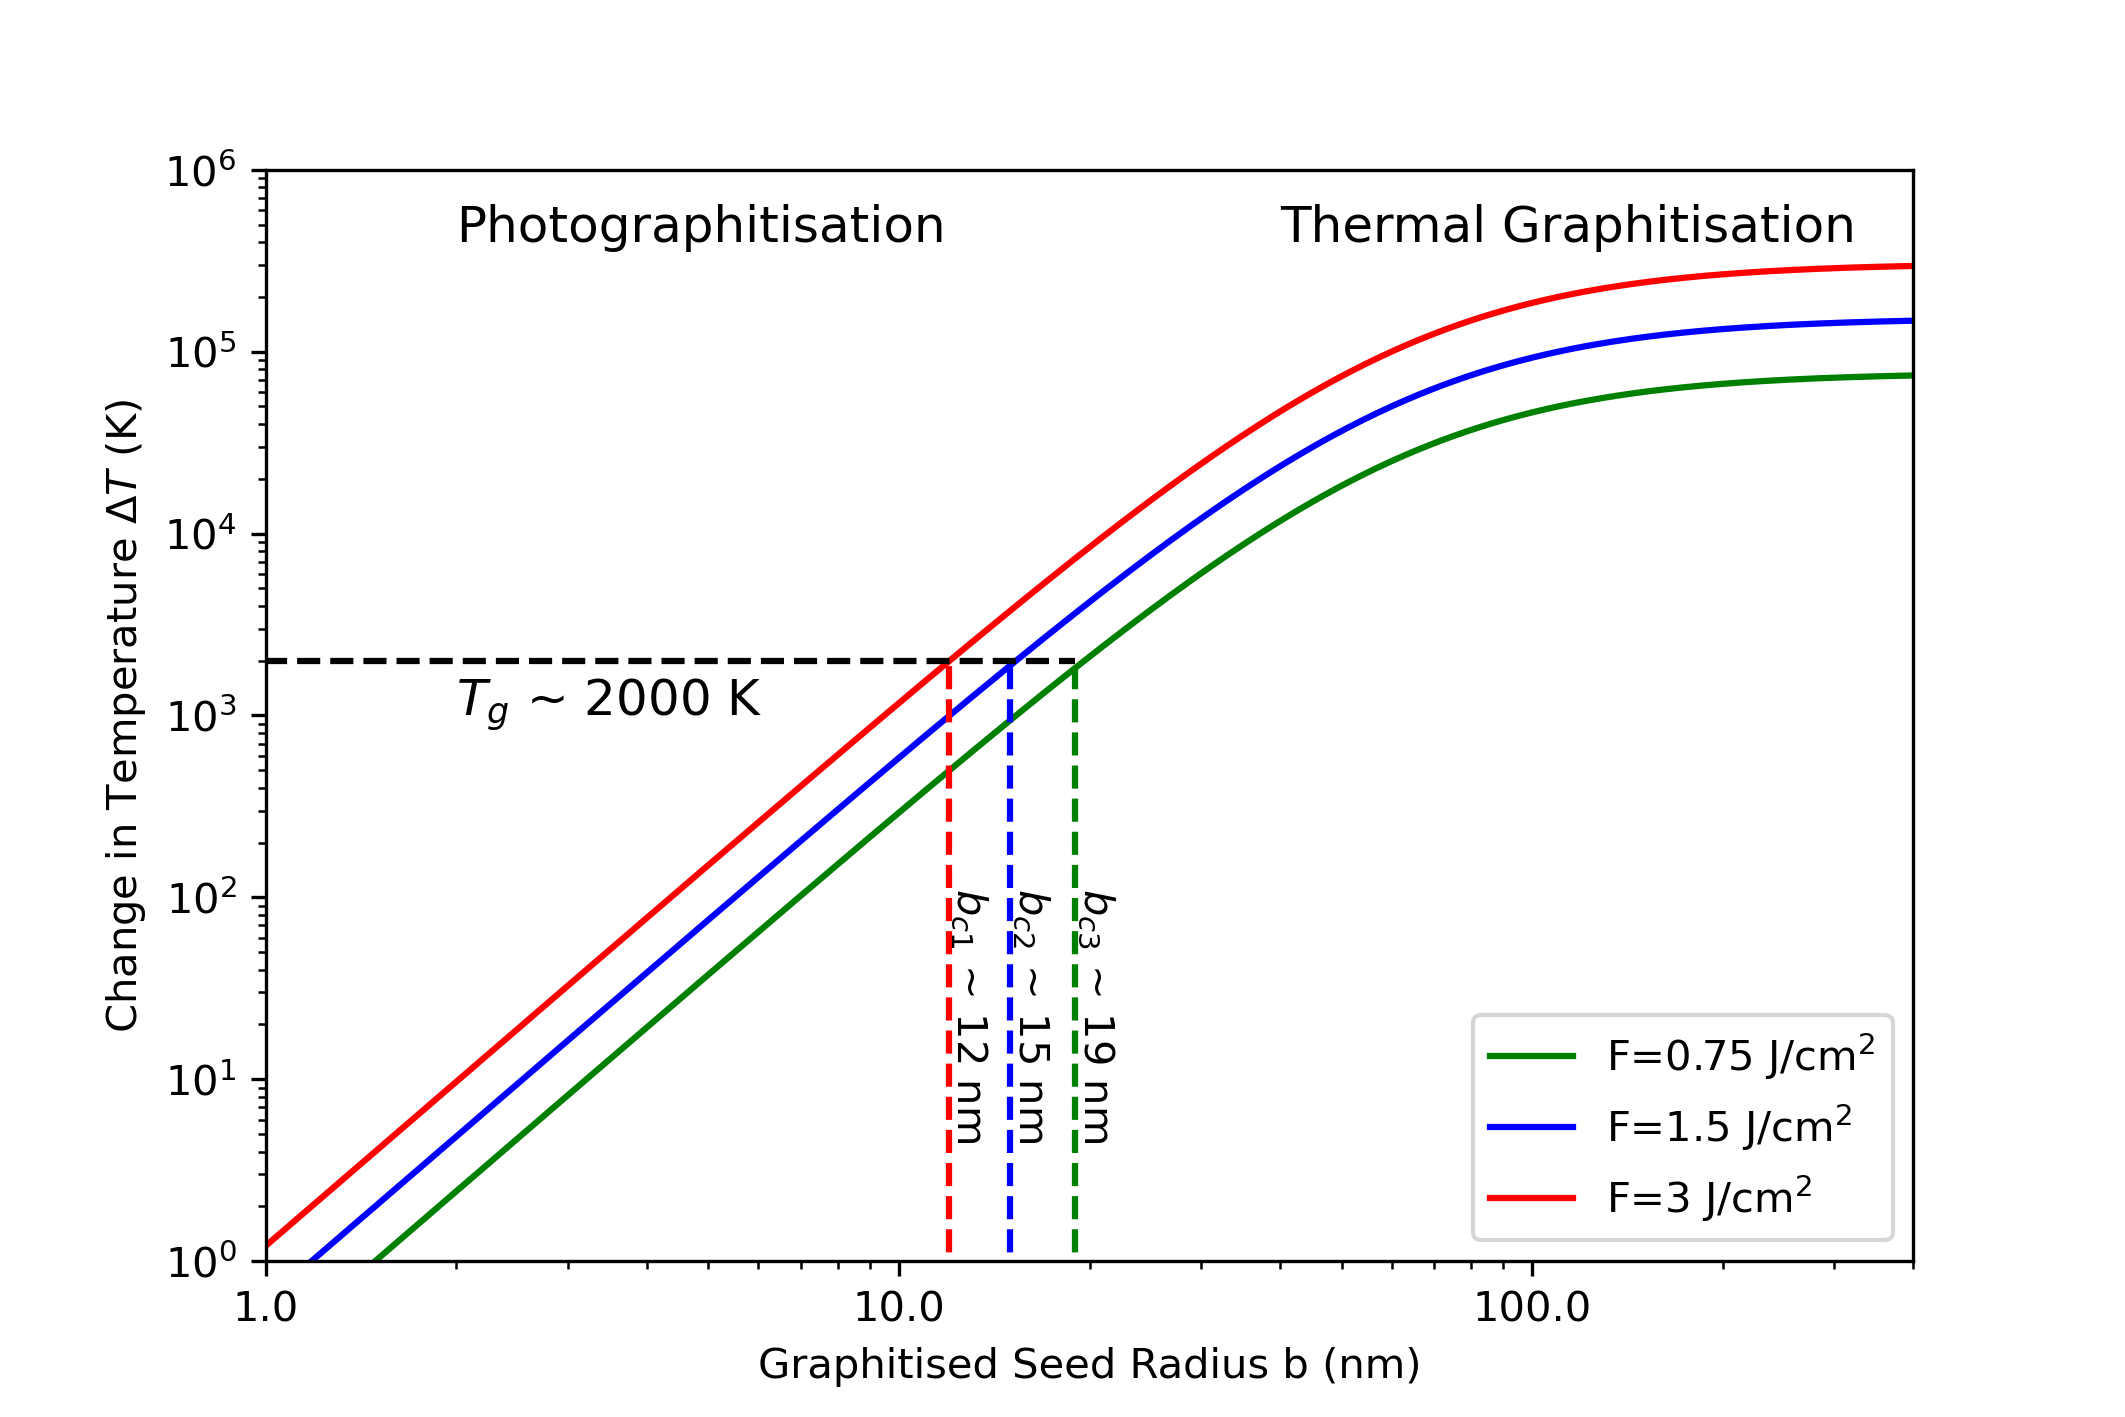
\includegraphics[width=\linewidth]{Chapter2/Figs/Raster/laser heating.png}
	\caption{The estimated laser-induced heating according to the model presented by Kononenko et al, represented by equations \ref{eq:deltaT}, \ref{eq:sigma laser}, \ref{eq:ld laser} at fluencies from $0.75$ \si{\joule\per\centi\metre\squared} to $3$ \si{\joule\per\centi\metre\squared}.}
	\label{fig:laser-heating}
\end{figure}

The critical seed radius at which thermal graphitisation becomes possible is marked as $b_{c1,2,3}$ for the three different fluencies respectively. It can be noted that at a lower laser fluence, a larger critical radius is calculated as the fluencies $0.75$, $1.5$ and $3$ \si{\joule\per\centi\metre\squared} resulted in a calculated critical radius of $19$, $15$ and $12$ \si{\nano\metre} respectively. This can be compared to figure \ref*{fig:fluencevsshots}, in which the number of laser pulse "shots" required for experimentally observed graphitisation is plotted against the laser fluence. This comparison is represented in figure \ref{fig:comparisonshots}. It is possible to infer a few points from this comparison, as the natural conclusion of lower fluence laser pulses requiring a larger critical radius also demands a larger number of laser shots to observe experimental graphite growth. This fits the model well, as the photographitisation step of adding layers to the graphitic defects will take far longer than the thermal graphitisation step. Indeed, this manifests as the requirement for an order of magnitude more laser pulses at merely half the laser fluence. It is hoped that under a certain fluence, the critical radius will be reduced to the scale of sub-microns and such will never be able to reach the thermal graphitisation stage of growth. Hence, the only graphitisation mechanism will be that of photographitisation at very low laser fluencies.

\begin{figure}
	\centering
	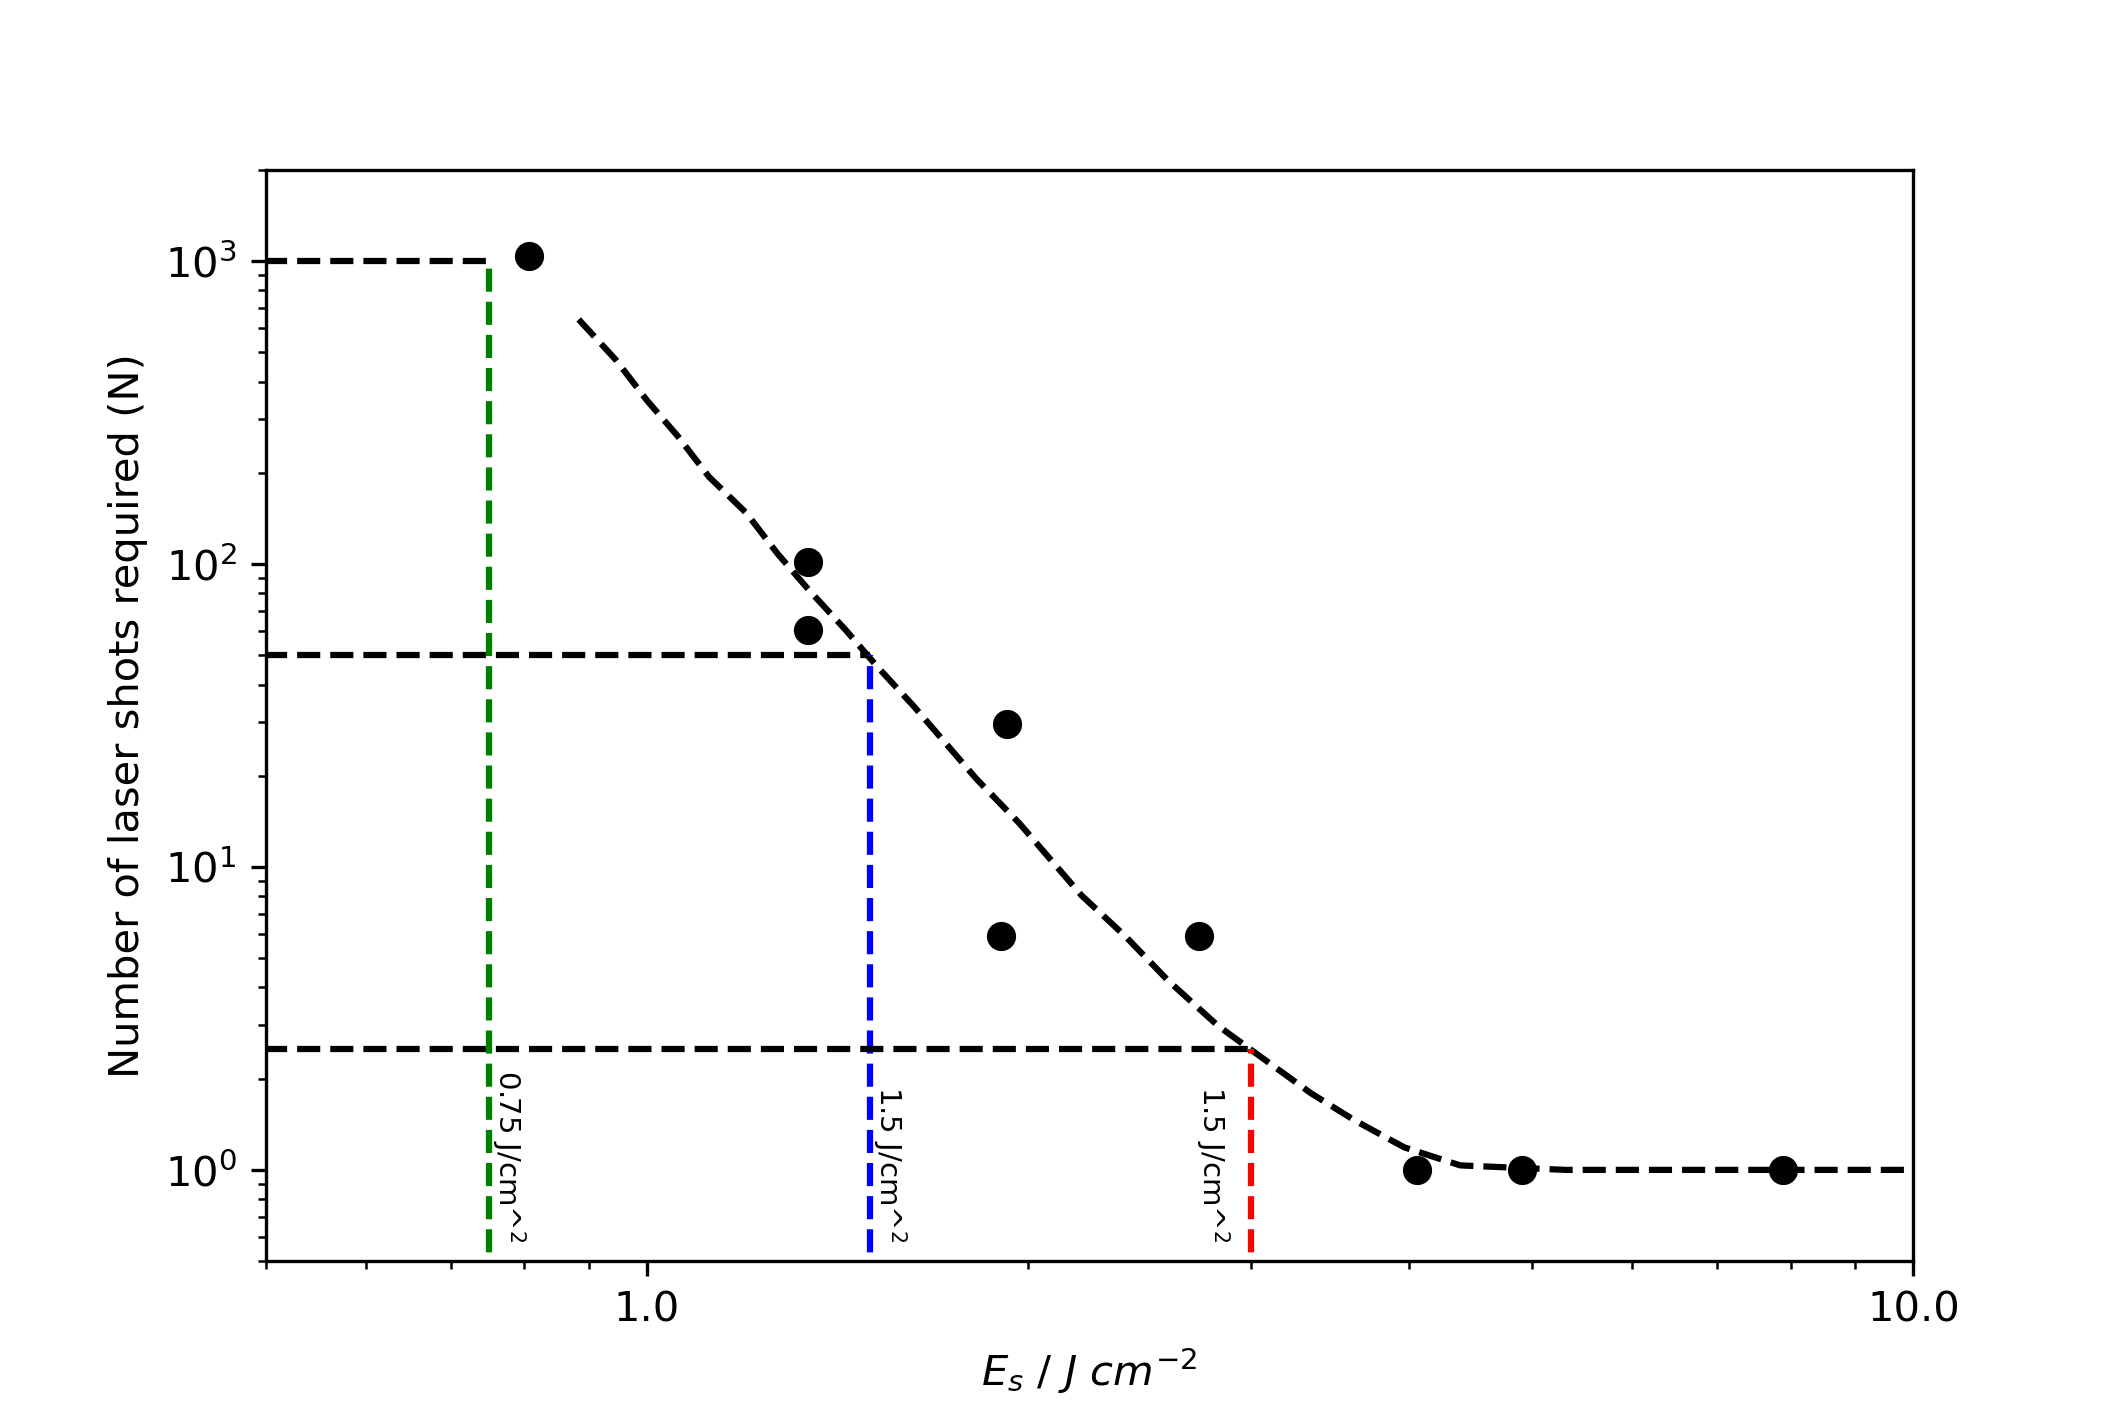
\includegraphics[width=\linewidth]{Chapter2/Figs/Raster/comparisonshots.png}
	\caption{A comparison of the laser fluencies used in the calculation of critical seed radii and the observed number of laser shots required for the process of graphitisation. The lower fluence requires a larger seed radius for thermal graphitisation and hence requires many more laser pulses for the photographitisation growth.}
	\label{fig:comparisonshots}
\end{figure}

\subsection{Graphite}
Graphite is typically manufactured by pressing or extruding a mixture of carbon containing materials such as pitch, coal, petrochemicals or other high molecular weight hydrocarbon, followed by a super-heating bake at anywhere from 2000 \si{\degreeCelsius} to more than 4000 \si{\degreeCelsius} to crystallise the amorphous carbon precursors. 

This heating is typically a multi-stage process, with the first step requiring a long, complex heating in vacuum of the carbon containing material to convert it into coke. This process is known as destructive distillation, with a "good coke" containing a very high carbon content and few if any impurities. The coke is then calcinated, crushed and sieved to obtain a certain distribution of particle sizes. These particles are then bound with a binding substance such as coal tar pitch, petroleum pitch or a synthetic resin and extruded or moulded to form the graphite products. Next, a carbonisation bake at around $1000\text{--}1200\si{\degreeCelsius}$ will thermally decompose the binder into elementary carbon and other volatile components, binding the powdered graphite together. The resulting volume of the formed carbon is lower than that of the binder, due to the formation of pores, with a relative volume or porosity depending upon the binder quantity.

Finally, the shaped and carbonised parts can be baked in the absence of oxygen, or in vacuum, at very high temperatures to induce crystallisation of the amorphous precursor carbon. Typical operating temperatures are in the $2500\text{--}3000\si{\degreeCelsius}$ range, which will also purify the graphite parts due to the vaporisation of impurities such as any remaining binder residue, oxides or gases. This is usually achieved with either induction based heating, or passing electric currents directly through the parts to utilise Joule heating.

A variety of precursors can be used, with gilsocarbon being a common choice for usage in nuclear power plants \cite{liu2017}.

It is also possible to form graphite via chemical vapour deposition (CVD) techniques, which is known as pyrolitic graphite. This form of graphite will have a very low porosity, approaching the theoretical density of graphite, with correspondingly improved material properties in most other aspects too.

\section{Metal-Semiconductor Contacts}

\subsection{Image Force/Schottky Effect}
\label{subsec:image_force_effect_schottky_effect}
 Given a point charge q at a distance x from a conducting plate, an "image" surface charge of opposite polarity is induced in the plate, with an induced electric field that is equivalent in magnitude and opposite to the point charge \cite{Feynman1965}. The force exerted on the "real" point charge is the "image force", with a corresponding force of:

\begin{equation}
\label{eq:image_charge_pe}
    F = -\frac{q^{2}}{16\pi \epsilon_{0}x^{2}}
\end{equation}
 where q is the charge (typically the charge of an electron, though generally for the point charge it is the charge of the point charge), $\epsilon_{0}$ is the permittivity of free space and $x$ is the distance of the point charge from the conductive plate. When the point charge is an electron, with an external electric field $\vec{E}$ applied to the system, the total potential energy PE as a function of the distance is given by \cite{Schroder2006-sx}:
 \begin{equation}
 \label{eq:pe_image}
     PE(x) = -\frac{q^{2}}{16\pi \epsilon_{0}x} - q\vec{E}x
 \end{equation}

\begin{figure}[H]
    \centering
    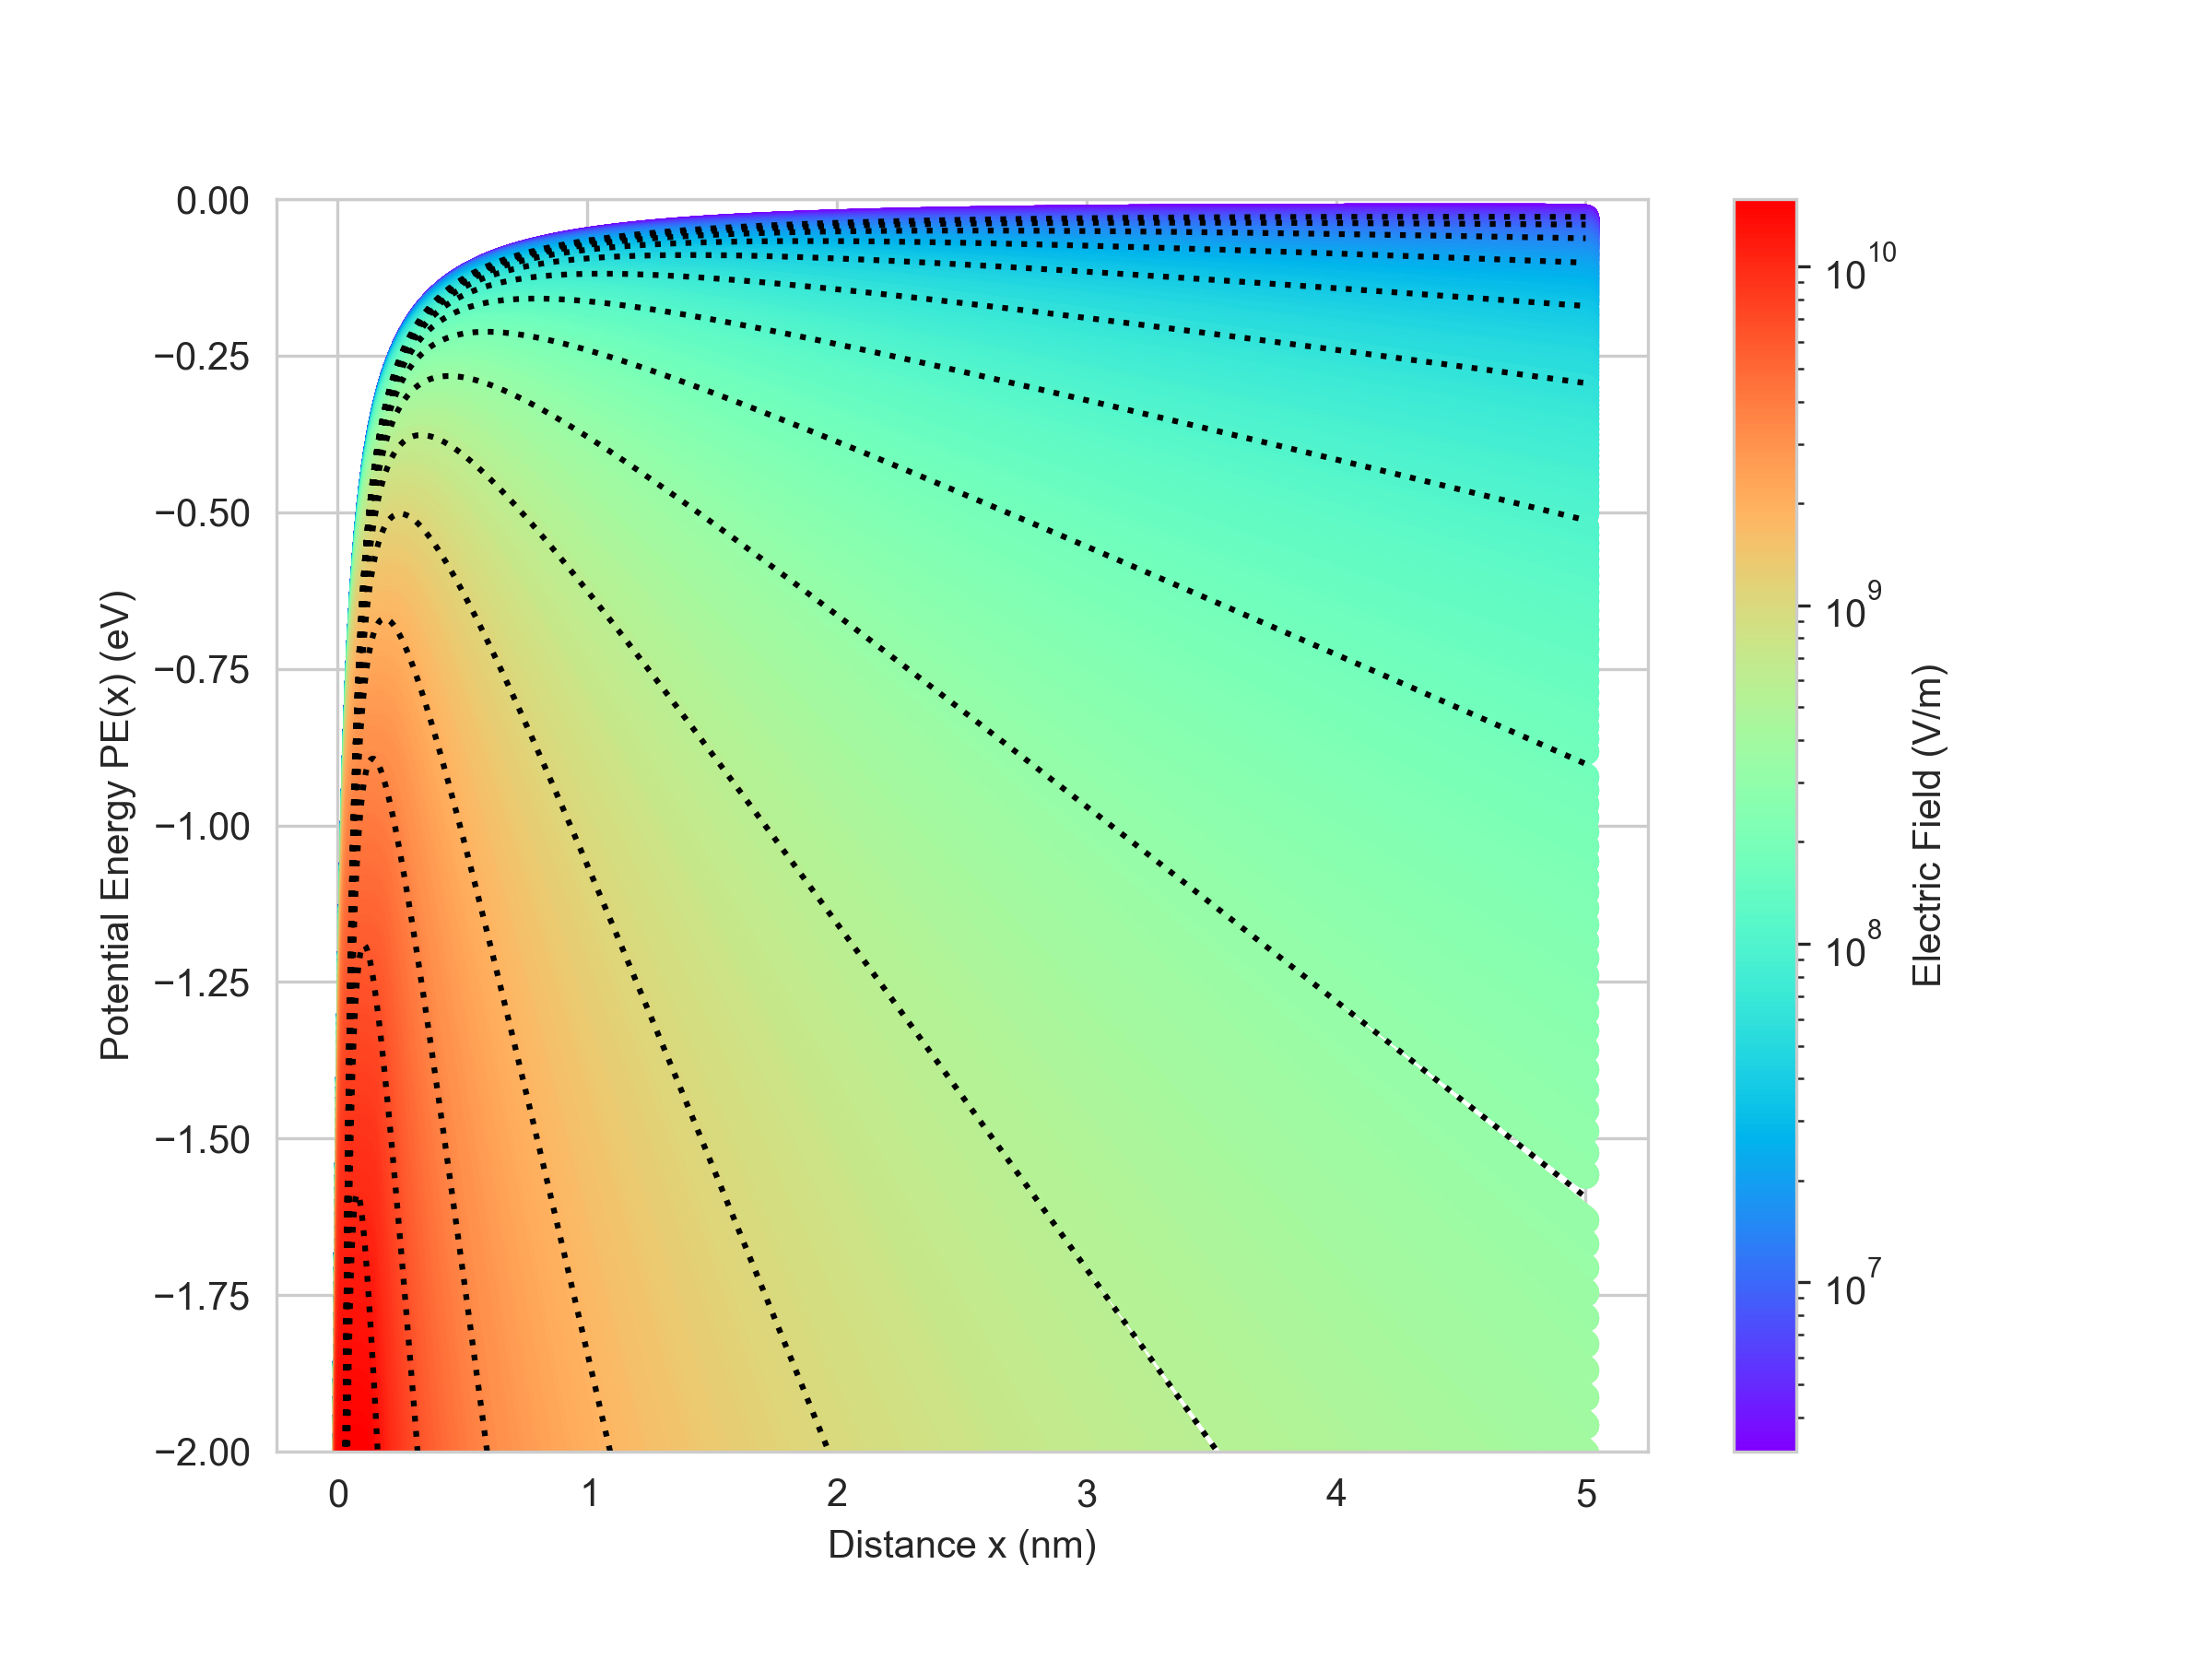
\includegraphics[width=\textwidth]{Chapter2/Figs/Raster/PE_image_charge_diamond.png}
    \caption{The potential energy of an electron due to the image charge effect at a metal-diamond boundary.}
    \label{fig:pe_image_charge}
\end{figure}

Figure \ref{fig:pe_image_charge} shows the application of equation \ref{eq:pe_image} to a range of high electric fields ($10^{6}$--$10^{10}$~\si{\volt\per\metre}. This visualisation uses a colour map to show the full spread of data, with black dotted lines for every quarter in the log scale. Very high electric fields form very sharp barriers, with heights substantially below the lower electric field Schottky curves. It should be noted that for lower electric fields below $10^{7}$~\si{\volt\per\metre}, the barrier lowering effect is much more slight, and is not possible to see on the scales used for this figure. Extension of this model in vacuum leads to the derivations of field effect emission, due to the possibility of quantum-mechanical tunnelling through these very thin high field barriers. The peaks of the barriers, or the point at which the rate of change of the potential energy barrier $\frac{d}{dx}(PE)$ is zero, are defined to be the position of $x_{m}$, which is where the barrier is shifted by an amount $\Delta\phi$ \cite{deVisschere1986, sze2006}:

\begin{equation}
\label{eq:image_force_barrier_lowering}
    \Delta \phi = \sqrt{\frac{q\abs{\vec{E}}}{4\pi\epsilon_{0}}} = 2\abs{\vec{E}}x_{m}
\end{equation}
\begin{equation}
    x_{m}= \sqrt{\frac{q}{16\pi\epsilon_{0}\abs{\Vec{E}}}}
\end{equation}
where $\vec{E}$ is a uniform electric field applied in the negative x direction of the conductor, determining the sign of $\Delta\phi$. 

When the metal-semiconductor interface is considered, the Debye length is crucial. If the semiconductor Debye length is much less than the range of the image force, of the order of \si{\angstrom}, then the semiconductor acts as a metal and equation \ref{eq:image_force_barrier_lowering} is used. The Debye length for semiconductors is given as \cite{sze2006}:

\begin{equation}
\label{eq:debye_length}
    L_{D}= \sqrt{\frac{\epsilon_{s}k_{B}T}{q^{2}N}}
\end{equation}
where N is either $N_{A}$ or $N_{D}$, depending upon whether the material is p or n-type respectively. When the Debye length is larger than the range of the image force, the semiconductor is considered to be a dielectric, and the modified form of image force barrier lowering is used for semiconductors:

\begin{equation}
    \label{eq:image_force_barrier_lowering_semiconductor}
    \Delta\phi = \sqrt{\frac{q\vec{E}_{m}}{4\pi\epsilon_{s}}}
\end{equation}

Where $\epsilon_{s}$ is the permittivity of the semiconductor, and the electric field within the semiconductor is not zero due to built-in potential bias. $\Vec{E}_{m}$ is the maximum value of the electric field at the semiconductor at the surface based on a depletion approximation \cite{sze2006}:

\begin{equation}
    \label{eq:max_e_field_depletion_approx}
    \vec{E}_{m} = \sqrt{\frac{2qN\abs{\Psi_{s}}}{\epsilon_{s}}}
\end{equation}

with surface potential $\Psi_{s}$ defined for ideal barrier heights $\phi_{Bn0}$ on n-type semiconductors:
\begin{equation}
    \label{eq:surface_potential}
    \abs{\Psi_{s}}= \phi_{Bn0}-\phi_{n}+V_{R}
\end{equation}

Finally, the Schottky effect for metal contacts to n-type semiconductors under differing biasing conditions is given as:
\begin{equation}
    \label{eq:schottky_effect_or_image_force_barrier_lowering_n-type_semi}
    \Delta\phi = \sqrt{\frac{q\vec{E}_{m}}{4\pi\epsilon_{s}}} = \left[ \frac{q^{3}N_{D}\abs{\Psi_{s}}}{8\pi^{2}\epsilon_{s}^{3}} \right]^{1/4}
\end{equation}

\begin{figure}[H]
    \centering
    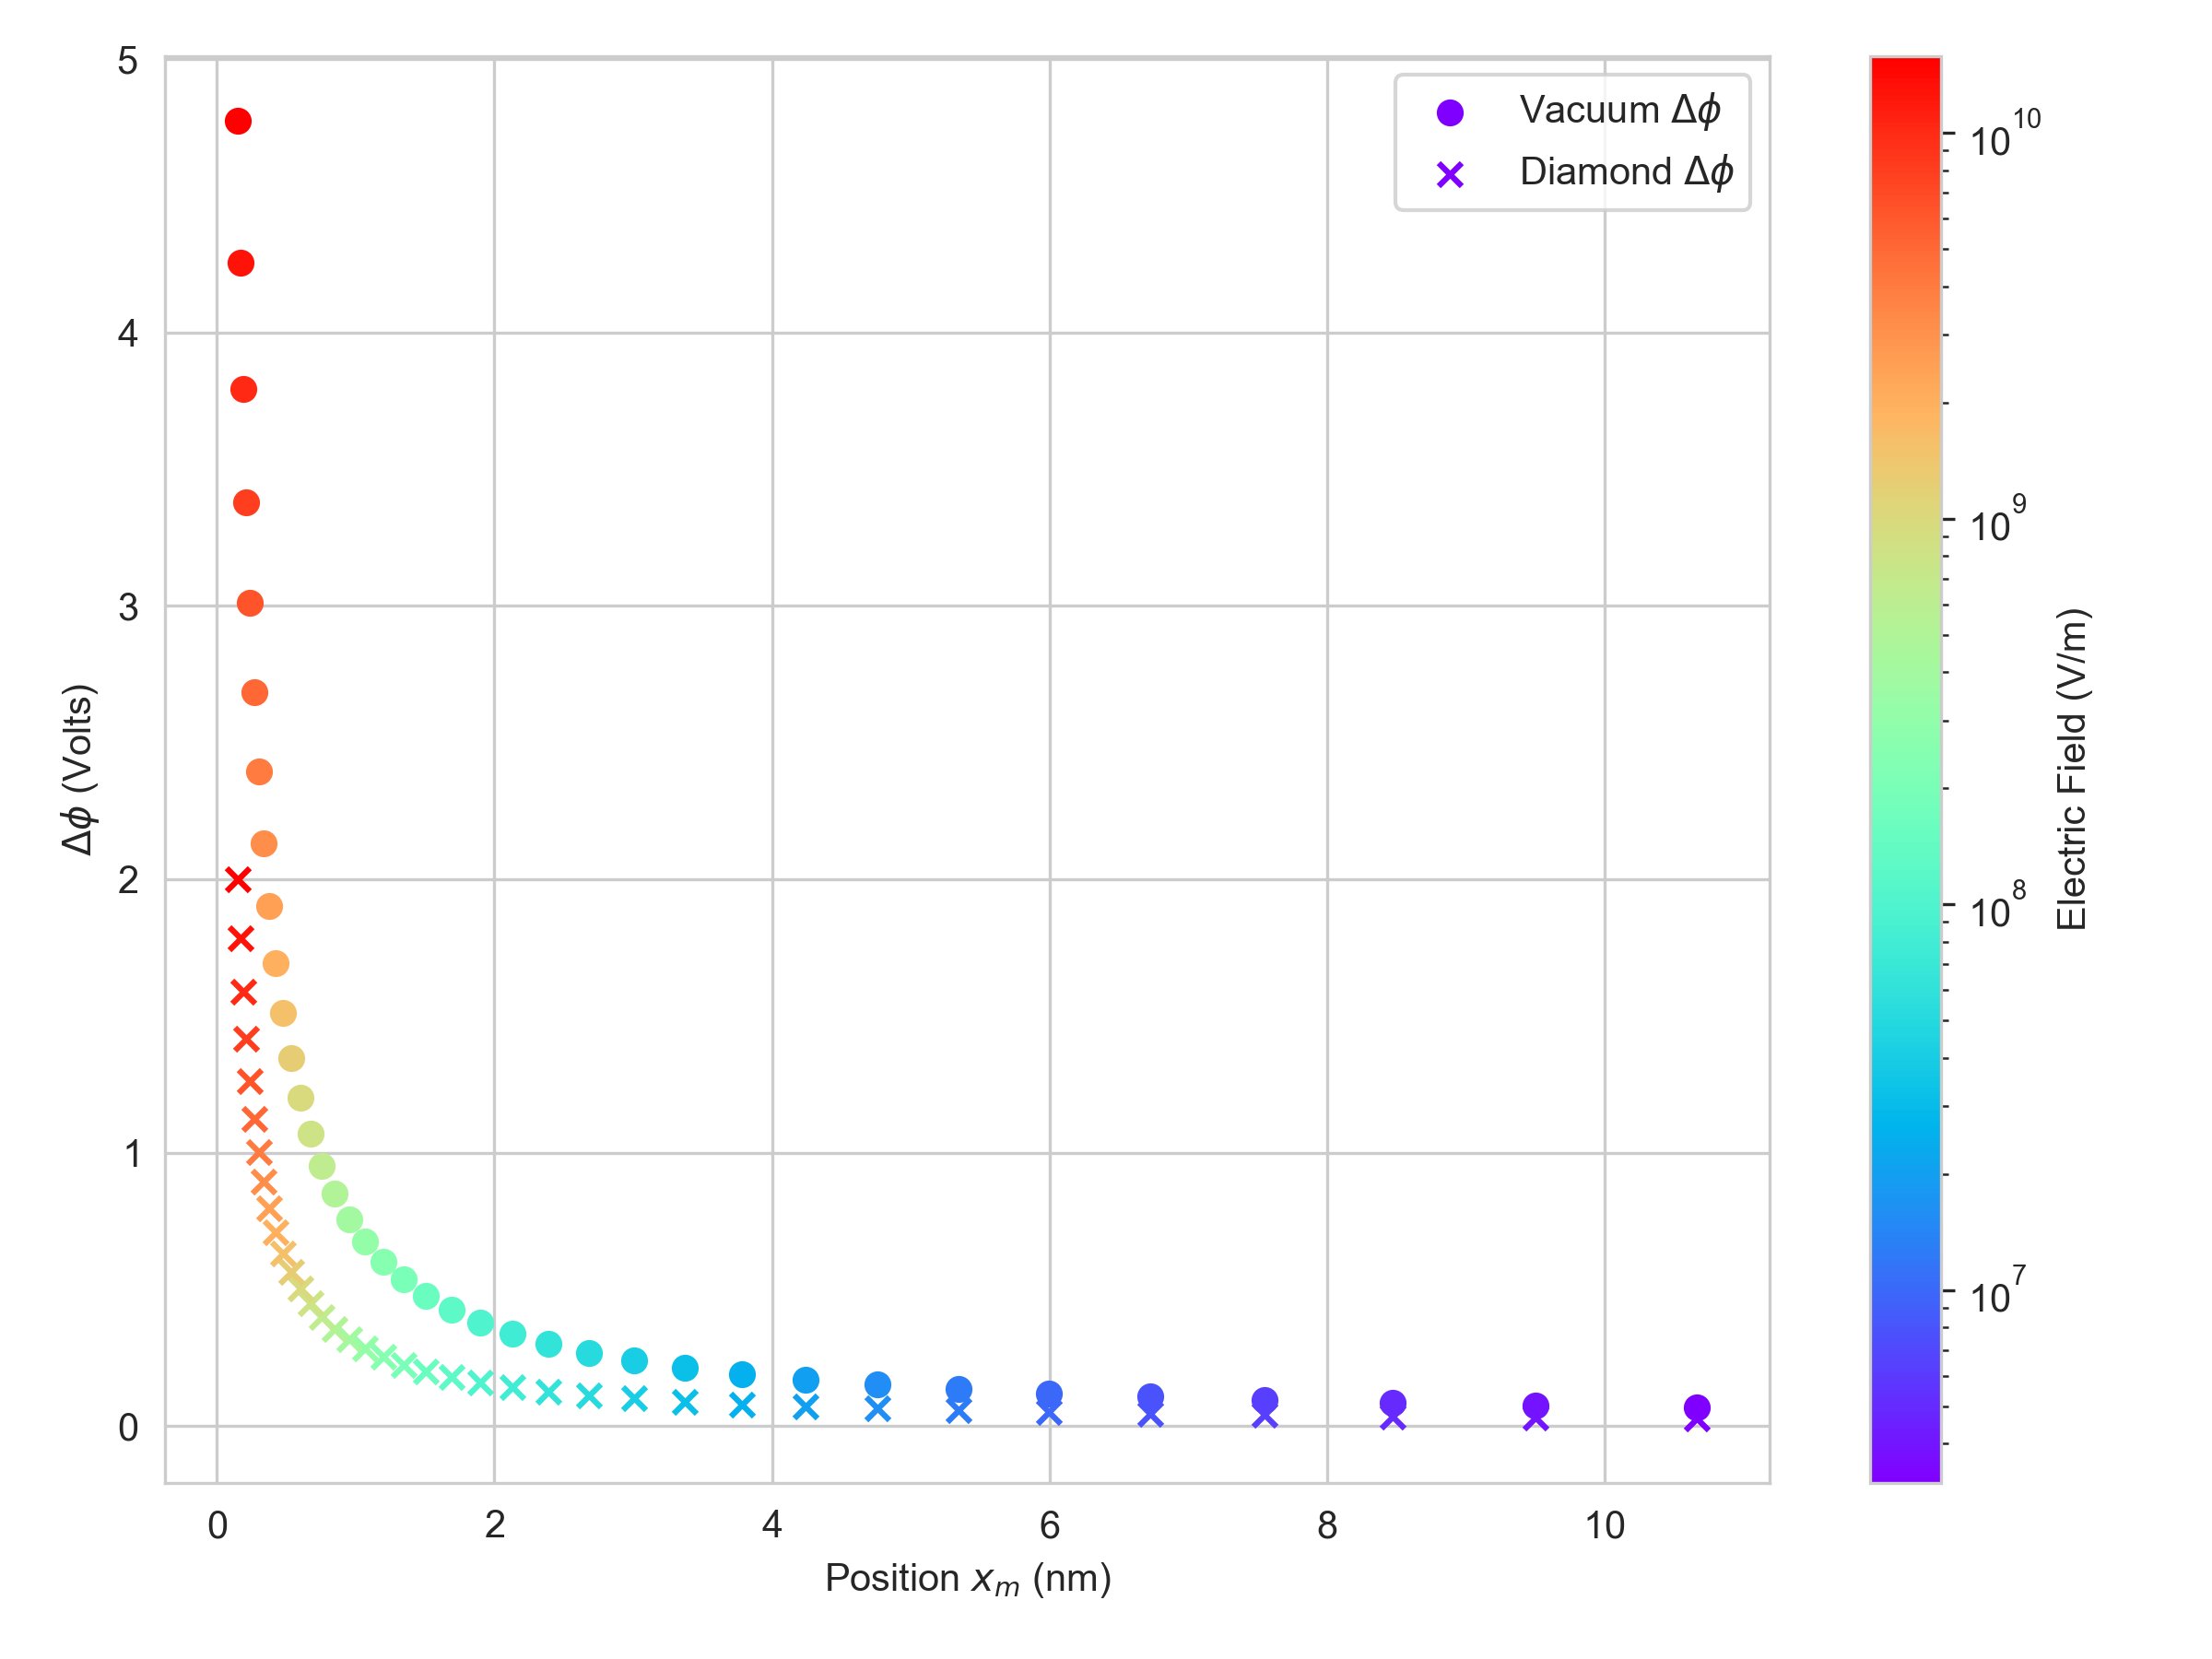
\includegraphics[width=\textwidth]{Chapter2/Figs/Raster/barrier_lowering_image_charge.png}
    \caption{The position and magnitude of the image force reduction of Schottky barrier height for metal-vacuum and metal-diamond.}
    \label{fig:pe_image_charge_reduction}
\end{figure}

Figure \ref{fig:pe_image_charge_reduction} presents a visual application of equation \ref{eq:image_force_barrier_lowering} and \ref{eq:schottky_effect_or_image_force_barrier_lowering_n-type_semi}. The resulting magnitude and location of the image force or Schottky effect can be seen for both the case of a metal in a vacuum, and that of an ideal metal and n-type diamond boundary with relative dielectric constant of 5.7 within the diamond \cite{Fontanella1977, Zaitsev2010-vd}.

\subsection{Double Schottky/Back-To-Back Schottky Estimation}
The mathematical formulation of double Schottky barriers depends upon a few key assumptions, with different levels of complexity depending upon the number of physical assumptions taken for the device structure. First, the most pressing question is whether or not the two Schottky barriers $\phi_{B}$ are equal. Next, the ideality factor for the two barriers may also differ. Finally, the mechanism for electron transport across the barrier must also be considered. While the ideality factor is used to generally account for additional electron emission into the semiconducting region, once the characteristic energy $E_{00}$ is significant, thermionic field emission or field emission alone may dominate and the thermionic emission of electrons across a Schottky barrier is no longer the prevailing mechanism. 

The double Schottky current density in the case of constant ideality factor between the two barriers is taken to be of the form \cite{Nouchi2014, Tang2006, Chiquito2012, Molinari2008}:

\begin{equation}
    J = \frac{J_{S1}J_{S2}\sinh{\frac{qV_{MSM}}{2nk_{B}T}}}{J_{S1}\exp{-\frac{qV_{MSM}}{2nk_{B}T}} + J_{S2}\exp{\frac{qV_{MSM}}{2nk_{B}T}}}
    \label{eq:double_schottky_j}
\end{equation}

\noindent where $q$ is the electron charge, $V_{MSM}$ is the voltage across the full metal/semiconductor/metal junction, $n$ is the ideality factor, $k_{B}$ is the Boltzmann constant and $T$ is the temperature. $J_{S1}$, $J_{S2}$ are the reverse saturation current densities across the first and second Schottky barriers respectively, as given by:

\begin{equation}
    J_{S1,S2} = A^{*}T^{2}e^{-\frac{\phi_{B01,2}}{k_{B}T}}
    \label{eq:reverse_saturation_j}
\end{equation}

\noindent where $A^{*}$ is the effective Richardson constant and $\phi_{B01,2}$ are the ideal barrier heights with no image force lowering effect for barriers 1 and 2 respectively. The inclusion of image force lowering or the Schottky effect \cite{Monch2004} in equation \ref{eq:double_schottky_j} is given by:

\begin{equation}
    V_{MSM} = n_{high}^{eff}\left(\phi_{B2}^{o}-\phi_{B1}^{o}\right) = n_{high}^{eff}\Delta\phi_{B}^{o}
    \label{eq:vmsm_correction}
\end{equation}

\noindent where $n_{high}^{eff}$ is the effective ideality factor corresponding to the forwardly biased Schottky barrier and $\phi_{B1,2}^{o}$ are the image force lowered Schottky barrier heights for barriers 1 and 2 respectively at zero bias. In many instances, the double Schottky model

\printbibliography[heading=subbibliography]

\end{refsection}